% !TeX spellcheck = <none>
\chapter{Revisão Bibliográfica} \label{chap:chap2}

Neste capítulo é realizada uma revisão bibliográfica das interfaces áudio e vídeo existentes, em específico do HDMI, também sobre métodos de codificação/descodificação de sinais HDMI numa FPGA e ainda sobre ligações de alta velocidade em série e cuidados que se deve ter com as mesmas.

\section{Interfaces de transmissão de video/audio}

As interfaces de áudio e vídeo definem parâmetros físicos e interpretações dos sinais recebidos, segundo \cite{R004}. Para sinais digitais a interface acaba por definir não só a camada física mas também a camada de ligação de dados e principalmente a camada da aplicação. As características físicas do equipamento (elétrico ou ótico) incluem o número e o tipo de ligações necessárias, tensões, frequências, intensidade ótica e ainda o design físico dos conectores. Relativamente à camada de ligação de dados, esta define como os dados da aplicação serão encapsulados para que, por exemplo, possam ser sincronizados ou para fazer correções de erros. Por fim, a camada da aplicação define o formato do sinal de áudio e vídeo a ser transmitido, normalmente incorporando \textit{codecs} não específicos. No entanto, por vezes esta camada acaba por não definir em concreto o tipo de formato de dados deixando em aberto tal parâmetro para que se possa transmitir dados no geral (é o caso do HDMI). No caso dos sinais analógicos, todas as funções que existem para os sinais digitais definidas em três camadas, são representadas num único sinal.

No caso da transmissão de sinais de áudio e vídeo digital existem várias interfaces que passam a ser analisadas, segundo \cite{R004}:
\begin{itemize}
	\item \textbf{\textit{Display Port:}} utiliza um conector do tipo \textit{DisplayPort} e é o principal concorrente do HDMI. Esta interface define uma interconexão sem licenças que foi inicialmente desenhada para ser utilizada numa conexão entre o computador e o monitor do mesmo. O sinal de vídeo não é compatível com DVI ou HDMI, mas um conector \textit{DisplayPort} pode fazer passar estes sinais.
	\item \textbf{\textit{ IEEE 1394 “FireWire":}} utiliza um conector do tipo \textit{FireWire} ou i.LINK. Este protocolo de transferência de dados é principalmente utilizado em câmaras digitais, mas também em computadores e em transferências de sinal de áudio. Este tipo de interface é capaz de hospedar vários sinais no mesmo cabo entregando os dados nos devidos destinos.
	\item \textbf{\textit{HDMI (High Definition Multimedia Interface):}} utiliza um conector do tipo HDMI e é uma interface de transmissão de sinal áudio/vídeo comprimida para transmissão de sinal digital descomprimida. 
\end{itemize}

\section{HDMI (\textit{High Definition Multimedia Interface})}\label{sec:HDMI}
O HDMI é uma interface de áudio e vídeo de alta definição que transporta dados áudio no formato não comprimido. Suporta num único cabo qualquer formato de vídeo em diversas resoluções e desde 2004 tem vindo a sofrer algumas alterações que vêm melhorar o desempenho da interface. 

Esta interface está dividida em diversos canais de comunicação que implementam determinados protocolos, entre os quais se destacam as seguintes de \cite{R002}:
\subsection{DDC - \textit{Display Data Channel} } \label{subsec:DDC} 
É um conjunto de protocolos utilizado nas comunicações digitais entre um dispositvo de origem e um dispositivo final que permite a comunicação entre ambos. Estes protocolos permitem que o ecrã comunique com o seu adaptador quais os modos que consegue suportar e também que o dispositivo que liga ao ecrã consiga ajustar alguns parâmetros, como por exemplo o contraste e a luminosidade. EDID (\textit{Extended display identification data}) é a estrutura \textit{standard} para este tipo de comunicações que define as capacidades do monitor e os modos gráficos suportados pelo mesmo.  Este protocolo é utilizado pela \textit{source} da comunicação do HDMI para obter os dados necessários do dispoistivo \textit{sink}, no sentido de perceber quais os modos suportados pelo mesmo. Este canal é também ativamente usado para HDCP (\textit{High-Bandwith Digital Content Protection}).

\subsection{TMDS - \textit{Transition-Minimized Differential Signaling} } \label{subsec:TMDS} 
É uma tecnologia utilizada para transmissão de dados em série de alta velocidade utilizado em comunicações digitais. O transmissor implementa um algoritmo que reduz as interferências eletromagnéticas nos cabos e permite ainda uma recuperação robusta de sinal de relógio no recetor. 

Em específico na interface HDMI, este protocolo divide a informação a transmitir em 3 principais pacotes e intercala a sua transmissão: Período de transmissão de vídeo, período de transmissão de dados e período de controlo. No primeiro período (período de transmissão de vídeo) são transmitidas os pixeis do vídeo em linha. No segundo período (o período de transmissão de dados) são transmitidos os dados de vídeo e os dados auxiliares à transmissão dentro dos respectivos pacotes. O terceiro período ocorre entre os dois anteriores. 

Para além de ser utilizada no HDMI, esta técnica é também utilizada em interfaces DVI.

\subsection{CEC - \textit{Consumer Electronics Control} } \label{subsec:CEC} 
É uma característica do HDMI que permite ao utilizador controlar até 15 dispositivos que tenham esta mesma característica ativa e que estão conectados por HDMI usando apenas um controlo remoto. Também é possivel dispositivos inviduais controlarem outros dispositivos sem intervenção do utilizador

\subsection{ARC - \textit{Audio Return Channel}  } \label{subsec:ARC} 
Esta característica do HDMI utiliza 2 pins do conector. É uma ligação de audio que tem como objetivo substituir outros cabos entre a TV e outros recetores ou então sistema de som. Esta direção é usada quando é a TV que gera ou recebe o vídeo mas é outro equipamente que reproduz o som. Esta característica está apenas disponível a partir da versão 1.4 de HDMI.

\subsection{HEC - \textit{HDMI Ethernet Channel}  } \label{subsec:HEC} 
Esta especificação do HDMI, tal como a anterior, está também apenas disponível a partir da versão 1.4 do HDMI e é uma tecnologia capaz de consolidar vídeo, audio e dados em série num único cabo HDMI, permitindo também aplicações baseadas em IP sobre o HDMI e uma comunicação \textit{Ethernet} bidireccional até 100 Mbit/s.

Uma das principais características mais recentes das interfaces HDMI prende-se ao facto de permitir que sinais não sejam reproduzidos em dipositivos não autrizados. Isto é, através de um protocolo cujo nome já foi referido anteriormente, HDCP (\textit{High-Bandwith Digital Content Protection}), o sinal HDMI pode ser encriptado e posteriormente transmitido pela \textit{source}, protegendo assim a sua reprodução em dispositivos não autorizados. Esta tem vindo a tornar-se uma característica importante, visto que a reprodução ilegal de vídeos tem vindo a tornar-se reccorrente nos dias atuais.

\section{Transmissão de dados HDMI}\label{sec:HDMIinFPGA}
A interface HDMI, tal como descrito no subcapítulo anterior, consiste numa interface que permite a transferência de sinais áudio e vídeo digitais entre dois dispositivos. Para que seja possivel a conexão entre dois dispositivos HDMI é necessário logo à partido que existam dois conectores HDMI, e ainda que o sinal que vem transportado no cabo seja descodificado para apenas serem transmitidos os dados referentes à imagem e ao som.   

O projeto recorre então à utilização de um tipo de \textit{hardware} capaz de cumprir as duas funções descritas, que são duas placas HDMI com o nome de TB-FMC-HDMI2.Ao todo são usadas duas placas, uma recetora do sinal HDMI (RX) e outra transmissora do sinal HDMI (TX) sendo que cada uma tem dois canais (RX0 e RX1, TX0 e TX1). No caso da placa recetora o sinal proveniente da fonte HDMI é recebido e, através dos conectores FMC, envia apenas os dados referentes à imagem e som. No caso da placa transmissora o processo é inverso, ou seja, os conectores FMC recebem os dados apenas referentes à imagem e ao som e a placa envia um sinal HDMI através do seu conector para o dispositivo final HDMI.

\subsection{Conexão à FPGA XILINX VC7203 Virtex-7} \label{subsec:HDMIconexao} 
Na figura~\ref{fig:fpgaVistaGeral} da página~\pageref{fig:fpgaVistaGeral}  visualiza-se a placa de desenvolvimento a ser utilizada no projeto. Assinalado a tracejado vermelho é possível visualizar os 3 conectores FMC (\textit{FPGA Mezzanine Card}) que a placa VC7203 disponibiliza.

\begin{figure}[h!]
	\begin{center}
		\leavevmode
		\includegraphics[width=1.0\textwidth]{fpga_fmc_vet}
		\caption{Vista Geral da FPGA VC7203 Virtex-7 retirada de \cite{R008}}
		\label{fig:fpgaVistaGeral}
	\end{center}
\end{figure}

%%DIZER AQUI QUE SÃO ESTES CONECTORES QUE SE VÃO LIGAR A FPGA
%%EXPLICAR EM QUE CONSISTEM OS CONECTORES FMC
Os conectores assinalados na imagem desta placa tratam-se de conectores FMC HPC (\textit{High Pin Count}) e permitem conectar as placas HDMI com a FPGA. Segundo \cite{R030}, os conectores FMC implementam determinadas normas que permitem uma rápida transmissão de dados entre placas. Exitem dois tipos de conectores FMC : LPC (\textit{Low Pin Count}) que disponibiliza 160 pinos e ainda HPC (\textit{High Pin Count}) que dispõe de 400 pinos. Ainda segundo \cite{R030}, qualquer tipo dos conectores consegue alcançar uma velocidade de conexão de até 2 Gb/s para sinais com sinalização diferencial e única. Para além da rápida velocidade de transmissão, outra gande vantagem que a utilização deste tipo de conectores traz é número de conexões que permite (400 pinos no caso de HPC) para a pequena area que ocupam. 
%%ESPECIFICAR QUANTO E QUE PARES SÃO DISPONIBILIZADOS

Em especifico nesta FPGA existem 3 conectores FMC (FMC1, FMC2 e FMC3) que permitem diferentes conectividades. Segundo \cite{R008}, o conector FMC1 dispões de 68 pares diferencias definidos pelo utilizador e ainda 4 sinais de relógio diferenciais. O mesmo acontece para para o conector FMC2. No entanto, o conector FMC3 apenas disponibiliza 65 pares diferencias que podem ser definidos pelo utilizador e 4 sinais de relógio diferencias.

Estes serão os conectores a ser utilizados e mais à frente neste relatório será explicado como é que os sinais são transmitidos. 


%A numeração 27, 28 e 29 correspondem aos conectores FMC disponíveis na FPGA a ser utilizada neste projeto. O número 27 corresponde ao conector JA2, 28 corresponde ao JA3 e 29 corresponde ao JA4. Estes conectores são usados como entradas e saídas de uma ligação, que neste caso em especifico será a uma placa HDMI, pois permitem uma ligação de alta velocidade (até 10 Gb/s). Estes três conectores HPC (High Pin Count) são compostos por 10x40 posições que permitem uma comunicação de alta velocidade por uma I/O cujo tamanho é relativamente pequeno. 
%
%\textbf{O conector JA2 (FMC1 HPC) permite a seguinte conectividade:}
%\begin{itemize}
%	\item 68 pares que podem ser definidos pelo utilizador:
%	\begin{itemize}
%		\item 34 pares LA
%		\item 17 pares HA
%		\item 17 pares HB
%	\end{itemize}
%	\item 4 sinais de relógio diferenciais
%\end{itemize}
%\textbf{O conector JA3 (FMC2 HPC) permite a seguinte conectividade:}
%\begin{itemize}
%	\item 68 pares que podem ser definidos pelo utilizador:
%	\begin{itemize}
%		\item 34 pares LA
%		\item 17 pares HA
%		\item 17 pares HB
%	\end{itemize}
%	\item 4 sinais de relógio diferenciais
%\end{itemize}
%\textbf{O conector JA2 (FMC1 HPC) permite a seguinte conectividade:}
%\begin{itemize}
%	\item 65 pares que podem ser definidos pelo utilizador:
%	\begin{itemize}
%		\item 34 pares LA
%		\item 16 pares HA
%		\item 15 pares HB
%	\end{itemize}
%	\item 4 sinais de relógio diferenciais
%\end{itemize}



\subsection{Recetor} \label{subsec:RX}

Na figura~\ref{fig:HDMIblocosRX} na página~\pageref{fig:HDMIblocosRX} é possível visualizar o diagrama de blocos do recetor.

\begin{figure}[h!]
	\begin{center}
		\leavevmode
		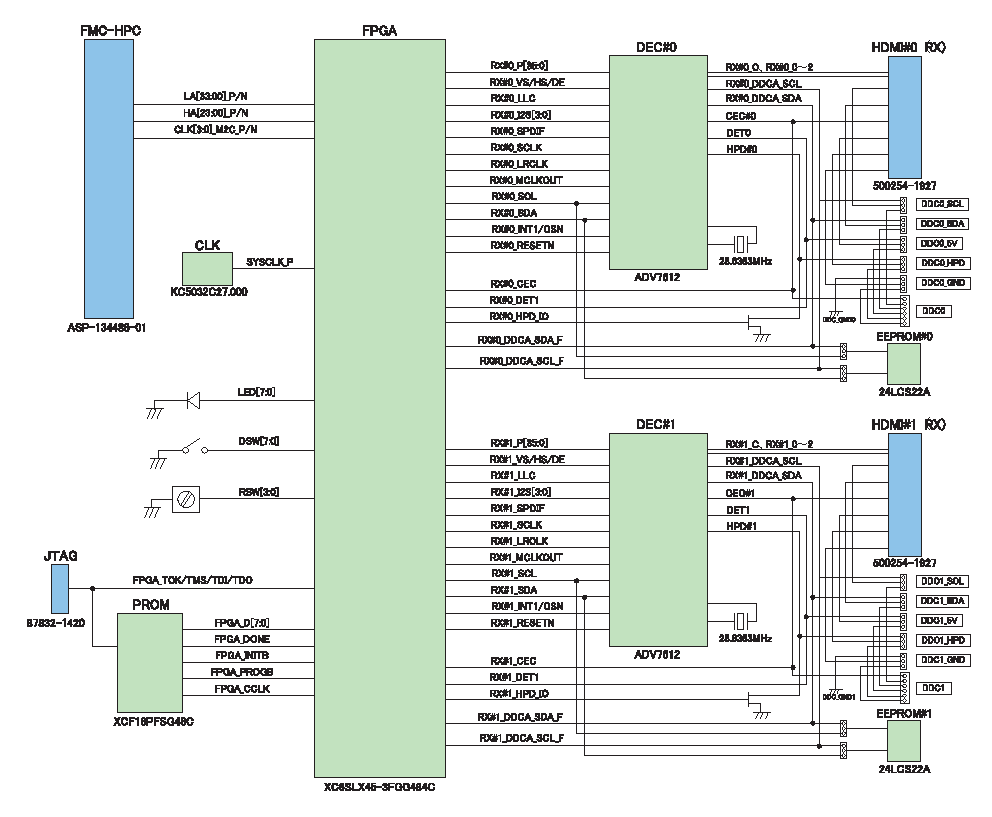
\includegraphics[width=1.0\textwidth]{diagramaBlocosRX_hdmi}
		\caption{Diagrama de blocos de TB-FMCH-HDMI2 RX retirado de \cite{R009}}
		\label{fig:HDMIblocosRX}
	\end{center}
\end{figure}
Através  de uma rápida observação deste diagrama é possivel concluir que se pode dividir as suas principais funções em duas partes que passa a ser descritas nos próximos sub-capitulos. 

\subsubsection{Receção do Sinal HDMI (ADV7612 para a FPGA localizada na placa)}
	
A receção do sinal HDMI é feita por um conector HDMI e usa um circuito integrado ADV7612BSWZ-P que recebe sinal HDMI e retira do mesmo os sinais a serem passados para a FPGA localizada na placa HDMI. O recetor tem também uma memória EEPROM (electrically erasable programmable read-only memory) que é usada para guardar dados EDID.
	
\subsubsection{Interface com o conector FMC (da FPGA localizada na placa para o conector FMC)}

Após passarem pela FPGA embebida na placa são passados os seguintes sinais presentes na tabela~\ref{table:HDMIdataRX} da página~\pageref{table:HDMIdataRX} (para o caso em que a FPGA está configurada por \textit{default}):

\begin{table}[h!]
		\fontfamily{cmr}\selectfont	
			\centering
			\resizebox{\textwidth}{!}{ 
			
			\begin{tabular}{@{}lllll@{}}
			\toprule
			{\textbf{Nome do Pin}} & {\textbf{\textit{Input/Output}}} & {\textbf{FPGA para FMC}}& {\textbf{FMC para FPGA}}       \\ \midrule  
			CLK0\_M2C\_P         & \textit{Output}                & RX\#0\_LLC             & RX\#0 sinal LLC                \\ 
			CLK1\_M2C\_P         & \textit{Output}                & RX\#1\_LLC             & RX\#1 sinal LLC                \\ 
			LA00\_P\_CC          & \textit{Output}                & RX\#0\_VSYNC           & RX\#0\_VSYNC                   \\ 
			LA01\_P\_CC          & \textit{Output}                & RX\#0\_HSYNC           & RX\#0\_HSYNC                   \\ 
			LA02\_P              & \textit{Output}                & RX\#0\_DE              & RX\#0 data enable              \\ 
			LA03\_P a LA32\_P    & \textit{Output}                & RX\#0\_P0 a RX\#0\_P29 & RX\#0 dados de vídeo de 0 a 29 \\ 
			LA33\_P              & \textit{Input/Output}          & Não usado              & ---------                     \\ 
			CLK0\_M2C\_N         & \textit{Input/Output}          & Não usado              & ---------                     \\ 
			CLK1\_M2C\_N         & \textit{Input/Output}          & Não usado              & ---------                      \\ 
			LA00\_N\_CC          & \textit{Output}                & RX\#1\_VSYNC           & RX\#1\_VSYNC                   \\ 
			LA01\_N\_CC          & \textit{Output}                & RX\#1\_HSYNC           & RX\#1\_HSYNC                   \\ 
			LA02\_N              & \textit{Output}                & RX\#1\_DE              & RX\#1 data enable              \\ 
			LA03\_N a LA32\_N    & \textit{Output}                & RX\#1\_P0 a RX\#1\_P29 & RX\#1 dados de vídeo de 0 a 29 \\ 
			LA33\_P              & \textit{Input/Output}          & Não usado              & ---------                     \\ 
			CLK2\_M2C\_P         & \textit{Input/Output}          & Não usado              & ---------                     \\ 
			CLK3\_M2C\_P         & \textit{Input/Output}          & Não usado              & ---------                     \\ 
			HA00\_P a HA23\_P    & \textit{Input/Output}          & Não usado              & ---------                     \\ 
			CLK2\_M2C\_N         & \textit{Input/Output}          & Não usado              & ---------                     \\ 
			CLK3\_M2C\_N         & \textit{Input/Output}          & Não usado              & ---------                     \\ 
			HA00\_N a HA23\_N    & \textit{Input/Output}          & Não usado              & ---------                     \\ \bottomrule	
		\end{tabular}}		
		\centering
		\caption{Nomes dos pins da interface FMC de TB-FMCH-HDMI2 RX, adaptada de \cite{R009}}
		\label{table:HDMIdataRX}
	\end{table}

Através da analise da tabela \ref{table:HDMIdataRX} e do diagrama de blocos da placa na figura \ref{fig:HDMIblocosRX} conclui-se que o integrado ADV7612 é capaz de colocar na sua saída vários sinais (tanto referentes à imagem como ao som), no entanto esses sinais não são todos transmitidos para os conectores FMC. Isto acontece por causa da configuração presente na FPGA embebida que determina que sinais envia para os conectores. 

Através da leitura de \cite{R016} conclui-se que a configuração presente na FPGA embebida para além de selecionar os dados a enviar para os conectores FMC, configura também alguns parâmetros do integrado ADV7612 que permitem que este reproduza sinais num determinado formato e com um determinado número de bits. 

Para esta configuração são transmitidos para os conectores dados FMC referentes à imagem e sinais de sincronização do mesmo. Os dados da imagem são enviados do recetor 0 entre os pinos LA03\_P a LA32\_P, e do recetor 1  entre LA03\_N a LA32\_P. O sinal “\textit{data enable}” é um sinal que sinaliza a chegada de dados e está ativo quando estão a ser transmitidos os sinais referentes a cada pixel. \textit{HSYNC} é um sinal que representa a sincronização horizontal e é um pulso que sincroniza o início da linha do dispositivo de destino com a imagem que a originou. Por outro lado, o sinal \textit{VSYNC} é a representação da sincronização horizontal, que faz o mesmo que \textit{HSYNC} (mas na vertical), certificando-se de que o dispositivo de destino começa no topo na imagem na altura correta.

Uma nota importante ainda sobre a passagem dos sinais através dos conectores FMC é que os dados provenientes da FPGA embebida na placa para os conectores são amostrados na transição de 1 para 0 do sinal de relógio do vídeo, e como tal, estes mesmos dados devem ser lidos na transição de 0 para 1 do sinal do relógio do lado da FPGA principal. A figura~\ref{fig:HDMIamostragemRX} na página~\pageref{fig:HDMIamostragemRX} ilustra esta situação.

\begin{figure}[h!]
	\begin{center}
		\leavevmode
		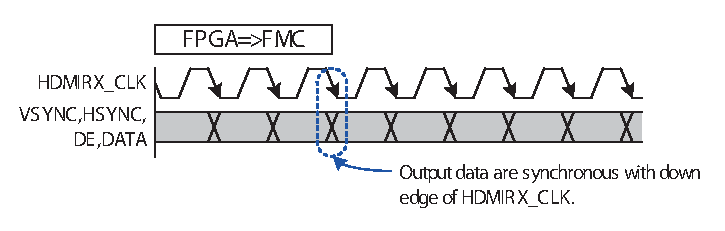
\includegraphics{amostragem_RX_vet}
		\caption{Amostragem dos dados provenientes da FPGA no recetor, retirada de \cite{R009}}
		\label{fig:HDMIamostragemRX}
	\end{center}
\end{figure}
 


\subsection{Transmissor}\label{subsec:TX} 

O diagrama de blocos do transmissor está representado na figura~\ref{fig:HDMIblocosTX} na página~\pageref{fig:HDMIblocosTX}.
\begin{figure}[h!]
	\begin{center}
		\leavevmode
		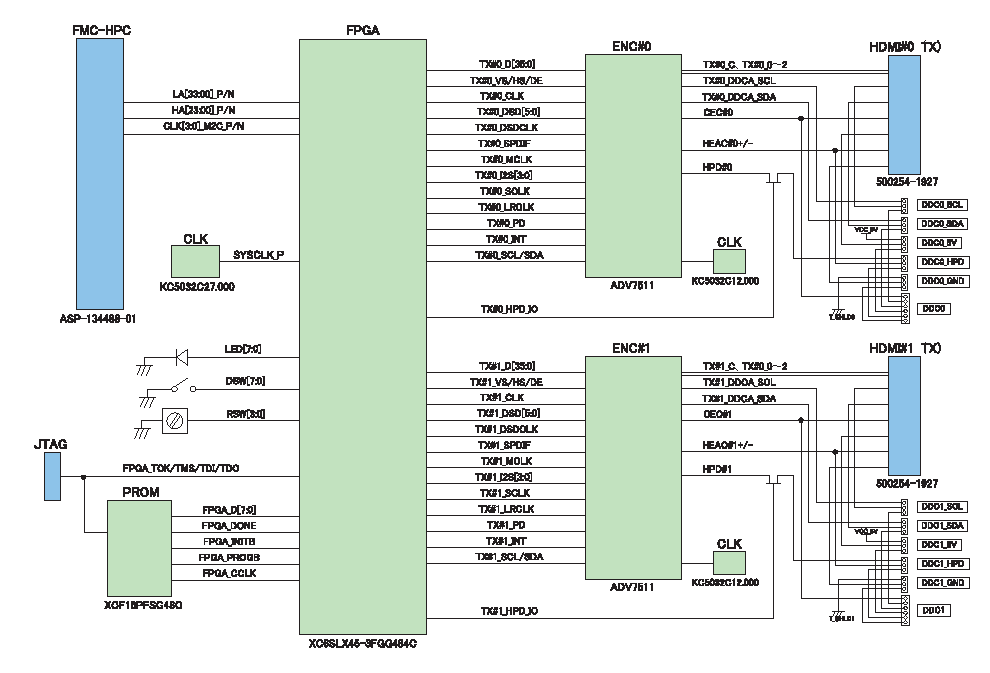
\includegraphics[width=1.0\textwidth]{diagramaBlocosTX_HDMI}
		\caption{Diagrama de blocos de TB-FMCH-HDMI2 TX retirado de \cite{R009}}
		\label{fig:HDMIblocosTX}
	\end{center}
\end{figure}
Mais uma vez é possível dividir o diagrama em duas principais funções que passam a ser descritas.

\subsubsection{Interface com o conector FMC (do conector FMC para a FPGA localizada na placa)}
No caso do transmissor o processo é feito no sentido inverso, ou seja, os sinais são lidos dos conectores FMC da placa HDMI e são amostrados para a FPGA embebida na mesma na transição de 0 para 1 do sinal de relógio do HDMI, tal como ilustra a imagem \ref{fig:HDMIamostragemTX} da página \pageref{fig:HDMIamostragemTX} e depois são processados pela FPGA de maneiraa a serem enviados para o transmissor HDMI (ADV7511).

	\begin{figure}[h!]
	\begin{center}
		\leavevmode
		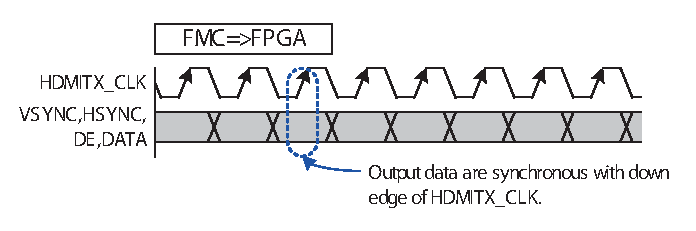
\includegraphics{amostragem_TX_vet}
		\caption{Amostragem dos dados provenientes do FMC no recetor, retirada de \cite{R009}}
		\label{fig:HDMIamostragemTX}
	\end{center}
\end{figure}

Os sinais representados na tabela~\ref{table:HDMIdataTX} na página~\pageref{table:HDMIdataTX} são equivalentes aos sinais presentes na tabela~\ref{table:HDMIdataRX} na página~\pageref{table:HDMIdataRX}, mais uma vez com a placa configurada por \textit{default}, e correspondem aos sinais que a placa transmissora deve receber para enviar para a FPGA.



\begin{table}[h!]
	\fontfamily{cmr}\selectfont	
	\centering
	\resizebox{\textwidth}{!}{ 	
		\begin{tabular}{@{}lllll@{}}
			\toprule
			\textbf{Nome do pin} & \textbf{Input/0utput} & \textbf{FMC para FPGA} & \textbf{FPGA para TX}          \\ \midrule
			CLK0\_M2C\_P         & Input                 & TX\#0\_DCLK            & TX\#0 sinal DCLK               \\ 
			CLK1\_M2C\_P         & Input/Output          & Não usado              & ----------                     \\ 
			LA00\_P\_CC          & Input                 & TX\#0\_VSYNC           & TX\#0\_VSYNC                   \\ 
			LA01\_P\_CC          & Input                 & TX\#0\_HSYNC           & TX\#0\_HSYNC                   \\ 
			LA02\_P              & Input                 & TX\#0\_DE              & TX\#0 data enable              \\ 
			LA03\_P a LA32\_P    & Input                 & TX\#0\_D0 a TX\#0\_D29 & TX\#0 dados de vídeo de 0 a 29 \\ 
			LA33\_P              & Input/Output          & Não usado              & ----------                     \\ 
			CLK0\_M2C\_N         & Input                 & TX\#1\_DCLK            & TX\#0 sinal DCLK               \\ 
			CLK1\_M2C\_N         & Input/Output          & Não usado              & ----------                     \\ 
			LA00\_N\_CC          & Input                 & TX\#1\_VSYNC           & TX\#1\_VSYNC                   \\ 
			LA01\_N\_CC          & Input                 & TX\#1\_HSYNC           & TX\#1\_HSYNC                   \\ 
			LA02\_N              & Output                & TX\#1\_DE              & TX\#1 data enable              \\ 
			LA03\_N a LA32\_N    & Output                & TX\#1\_D0 a TX\#1\_D9  & TX\#1 dados de vídeo de 0 a 29 \\ 
			LA33\_P              & Input/Output          & Não usado              & ----------                     \\ 
			CLK2\_M2C\_P         & Input/Output          & Não usado              & ----------                     \\ 
			CLK3\_M2C\_P         & Input/Output          & Não usado              & ----------                     \\ 
			HA00\_P a HA23\_P    & Input/Output          & Não usado              & ----------                     \\ 
			CLK2\_M2C\_N         & Input/Output          & Não usado              & ----------                     \\ 
			CLK3\_M2C\_N         & Input/Output          & Não usado              & ----------                     \\ 
			HA00\_N a HA23\_N    & Input/Output          & Não usado              & ----------                     \\ \bottomrule
		\end{tabular}}
			\caption{Nomes dos pins da interface FMC de TB-FMCH-HDMI2 TX, adaptada de \cite{R009}}
			\label{table:HDMIdataTX}
	\end{table}

%
%\newcolumntype{d}{D{.}{.}{2.3}}
%\newcolumntype{C}{>{\centering}p}
%	\begin{table}[]
%		\caption{Comparison of Elements in Air on the Space Station and sea level on Earth}    
%		\centering
%		\begin{center}
%			\begin{tabular}{p{1.25in}ddd}
%				\toprule
%				\multicolumn{1}{C{1.25in}}{Nome do Pin} & \multicolumn{1}{C{1in}}{Input/0utput} & \multicolumn{1}{C{1.25in}}{FMC para FPGA} &         \multicolumn{1}{C{1in}}{FPGA para TX}\\
%				\midrule
%				CLK0\_M2C\_P         & Input                 & TX\#0\_DCLK            & TX\#0 sinal DCLK               \\ 
%				CLK1\_M2C\_P         & Input/Output          & Não usado              & ----------                     \\ 
%				LA00\_P\_CC          & Input                 & TX\#0\_VSYNC           & TX\#0\_VSYNC                   \\ 
%				LA01\_P\_CC          & Input                 & TX\#0\_HSYNC           & TX\#0\_HSYNC                   \\
%				LA02\_P              & Input                 & TX\#0\_DE              & TX\#0 data enable              \\ 
%				LA03\_P a LA32\_P    & Input                 &  \multicolumn{1}{C{1in}}{}TX\#0\_D0 a TX\#0\_D29} & TX\#0 dados de vídeo de 0 a 29 \\ 
%				LA33\_P              & Input/Output          & Não usado              & ----------                     \\ 
%				CLK0\_M2C\_N         & Input                 & TX\#1\_DCLK            & TX\#0 sinal DCLK               \\ 
%				CLK1\_M2C\_N         & Input/Output          & Não usado              & ----------                     \\ 
%				LA00\_N\_CC          & Input                 & TX\#1\_VSYNC           & TX\#1\_VSYNC                   \\ 
%				LA01\_N\_CC          & Input                 & TX\#1\_HSYNC           & TX\#1\_HSYNC                   \\ 
%				LA02\_N              & Output                & TX\#1\_DE              & TX\#1 data enable              \\ 
%				LA03\_N a LA32\_N    & Output                & TX\#1\_D0 a TX\#1\_D9  & TX\#1 dados de vídeo de 0 a 29 \\ 
%				LA33\_P              & Input/Output          & Não usado              & ----------                     \\ 
%				CLK2\_M2C\_P         & Input/Output          & Não usado              & ----------                     \\ 
%				CLK3\_M2C\_P         & Input/Output          & Não usado              & ----------                     \\ 
%				HA00\_P a HA23\_P    & Input/Output          & Não usado              & ----------                     \\ 
%				CLK2\_M2C\_N         & Input/Output          & Não usado              & ----------                     \\
%				CLK3\_M2C\_N         & Input/Output          & Não usado              & ----------                     \\ 
%				HA00\_N a HA23\_N    & Input/Output          & Não usado              & ----------                     \\ 
%				\bottomrule
%			\end{tabular}
%		\end{center}
%		\label{default}
%	\end{table}
%	
	

	
\subsubsection{Transmissor HDMI (da FPGA localizada na placa para ADV7511)}

Os sinais são então processados de maneira a envia-los para o bloco ADV7511 localizado na placa. Através da analise dos documentos \cite{R017} e \cite{R018} conclui-se que para além dos dados de imagem e os seus sinais de controlo, são também enviados para o integrado ADV7511 alguns sinais de controlo que indicam ao integrado que tipo de formato de imagem são enviados, ou quantos números de bits tem, entre outras informações.De seguida, o ADV7511 converte o sinal para o poder enviar através do cabo HDMI para o dispositivo final. 



%\subsubsection{Conexão DDC}\label{subsubsec:DDCconexao} 
%
%Para esta configuração da placa, são suportadas dois tipos de conexão DDC que passam a ser descritas.
%
%\begin{enumerate}
%	\item \textbf{Conexão Normal}
%	
%	\hspace{1.0em}Nesta configuração a comunicação DDC realiza-se normalmente entre o recetor e o transmissor HDMI, tal como ilustra a figura~\ref{fig:DDCnormal} na página~\pageref{fig:DDCnormal}. Existe um canal especifico para esta conexão que é recebido através do conector HDMI e enviado juntamente com os outros tipos de dados.
%
%	\begin{figure}[h!]
%		\begin{center}
%			\leavevmode
%			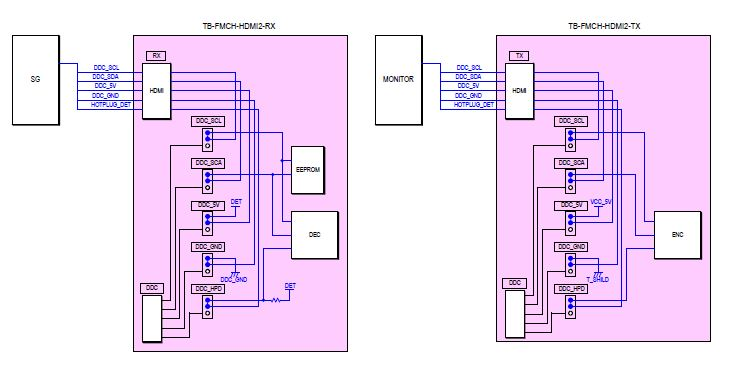
\includegraphics[width=1.0\textwidth]{DDCnormal}
%			\caption{Configuração DDC normal, retirada de \cite{R009}}
%			\label{fig:DDCnormal}
%		\end{center}
%	\end{figure}
%	
%	\item \textbf{Conexão "\textit{through}"}
%	
%	\hspace{1.0em}Este tipo de conexão faz uma ligação direta do canal DDC entre o recetor e o transmissor inibindo a comunicação normal deste canal. Para fazer esta conexão é necessário um cabo DDC e fazer as conexões corretas. Esta situação está ilustrada na figura~\ref{fig:DDCthrough} na página~\pageref{fig:DDCthrough}.
%	
%		\begin{figure}[h!]
%		\begin{center}
%			\leavevmode
%			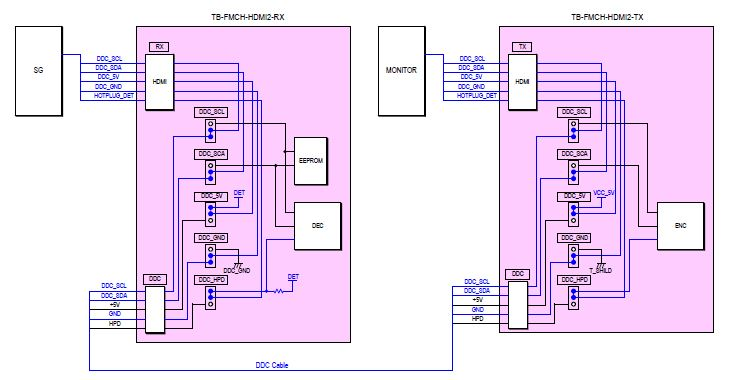
\includegraphics[width=1.0\textwidth]{DDCthrough}
%			\caption{Configuração DDC “\textit{through}”, retirada de \cite{R009}}
%			\label{fig:DDCthrough}
%		\end{center}
%	\end{figure}
%	
%	\hspace{1.0em}Este tipo de configuração poderá ser utilizada numa fase inicial do projeto a ser realizado, visto que não exige comunicação bidirecional através dos transcetores (onde os restantes sinais serão transmitidos), e como tal vem facilitar a comunicação entre dispositivo de origem e de destino.
%\end{enumerate}

%\section{Conexão de alta velocidade em série -> NOVO SUB-CAPITULO} \label{sec:conexaoSerie_new}
%
%A comunicação de dados de alta velocidade pode ser efetuada tanto em série como em paralelo, sendo que cada uma tem as suas devidas implicações. No caso das comunicações em paralelo é possivel atingir uma velocidade de comuncação maior, no entanto tem um custo mais elevado devido à necessidade de mais recursos físicos. Para além de um custo maior apresentam também 



\section{Conexão de alta velocidade em série} \label{sec:conexaoSerie}

Nesta secção será abordado o tema de comunicação em série em alta velocidade, desde as suas vantagens e desvantagens até tipos de arquiteturas habitualmente utilizados.

\subsection{Comunicações em paralelo VS comunicaões em série}

Desde sempre que tanto a comunicação em série como em paralelo têm vindo a ser utilizadas para as diferentes aplicações que envolvem a transmissão de dados entre modulos, e neste capitulo serão abordadas as diferentes características de cada um. A comunicação de dados em paralelo é utilizada para comunicações relativamente curtas pelo facto de ser mais simples e não trazer tantas implicações. Olhando para um exemplo em concreto deste projeto: a comunicação entre as placas HDMI e a FPGA VC7203 é feita em paralelo através dos conectores FMC, tal como explicado em \ref{subsec:HDMIconexao}, porque é uma distância bastante curta e não envolve preocupações no que toca a dobrar ou triplicar a freqência de transmissão e vice-versa. Afinal, para transmitir um determinado número de dados em série é necessário multiplicar esse número de dados pela frequência de transmissão em paralelo do lado do transmissor, e do lado do recetor é necessário lidar com eventuais desalinhamentos. 

Quando este tipo de comunicações começaram a ser utilizadas a distâncias maiores e a ser também necessário uma velocidade de comunicação maior, então começaram a haver mais problemas relativamente ao uso desta forma de transmissão. Apesar de, segundo \cite{R032}, terem sido aplicados métodos que viessem melhorar o desempenho destas comunicações em termos de velocidade, como por exemplo, a sinalização diferencial que veio aumentar a mesma, existem ainda bastantes desvantagens segundo \cite{R012}. Há uma  desvantagem que se torna banstante óbvia de constatar que é o custo: ter uma ligação em série com um cabo é muito menos dispendioso do que ter 400 cabos (no caso da transmissão entre as placas HDMI e a FPGA) para ter uma ligação em paralelo. Para além disto existem mais três problemas também apontados por \cite{R012} : \textit{clock skew}, \textit{data skew} e \textit{crosstalk}. \textit{Clock} e \textit{data skew} tratam-se de pequenos desvios na chegada ao recetor dos dados e dos sinais de relógio, isto porque nem todos são transmitidos exatamente à mesma velocidade e como tal podem provocar pequenos atrasos. Apesar de serem pequenos, podem vir a causar problemas visto que a velocidade de transmissão é bastante alta. Segundo este mesmo autor, existem já técnincas capazes de corrigir estes atrasos relativamente ao sinal de relógio (devido à sua perciocidade), e a correcção dos dados também é possivel, no entanto é muito mais problemática. A \textit{crosstalk} trata-se de uma interferência entre cabos adjacentes, inerente à transmissão, que se torna ainda mais problemática com o aumento dos mesmos.

%Falar das vantagens de usar comunicação em série
Estas razões, entre outras, têm vindo a motivar o desuso das comunicações em paralelo para transmisões de alta velocidade. Em \cite{R032} são mostradas algumas das razões para usar as ligações em série para tal efeito. O autor menciona o facto da utlilização de menos pinos para uma maior largura de banda, o que faz com que o custo da transmissão baixe consideravelmente. Este autor considera também um problema das transmissões em paralelo que não acontece em série: as consequências das constantes alternâncias das saídas. Isto é, numa ligação em paralelo o mais provável é que todas as saídas estejam a alterar constantemente e como tal esta alternância na massa acaba por criar ruído que é propagado na ligação. Claro que é possivel resolver este problema aplicando sinalização diferencial aos sinais transmitidos, mas em contrapartida aumenta o número de pinos necessários, aumentando por isso o custo da ligação.

%Desvantagens de usar comunicação em série
Aparantemente, torna-se obvio que as ligações em série devem ser usadas para este efeito uma vez que só acartam consigo vantagens, no entanto é necessário ter com consideração as desvantagens desta utilização. 

Logo à partida o primeiro problema que rapidamente o autor de \cite{R032} constata é a integridade do sinal, isto é, é expectável que para garantir a integridade do sinal será necessário recorrer a mais lógica que o garanta. Para além disso, também será de esperar que este tipo de comunicaçãos exiga placas, cabos e conectores de alta velocidade que são mais caros. E claro, uma vez que estas comunicações trabalham a uma cadência bastante elevada também de esperar que seja necessário fazer simulações digitais em bases de tempo mais pequenas o que pode trazer algumas complicações.
%Problemas na integridade do sinal
%Também podemos esperar para pagar mais por placas de PC controladas por impedância, conectores e cabos de alta velocidade.

Em conclusão, e tal como o autor de \cite{R032} menciona, hoje em dia a utilização de ligações em série já não são utilizadas apenas na indústria das telecomunicações mas acaba por ser transversal a outras trantas que a usam. O autor remata ainda que o futuro da eletrónica passa por comunicações em série.
%O autor de \cite{R032} menciona que hoje em dia este tipo de comunicações é usada não so na indústria das telecomunicações mas também numa vasta variedade de seccções e remata ainda que o futuro da eletrónica passa por comunicações em série. Este autor refere ainda que este tipo de comunicações pode vir a trazer vantagens em ligações \textit{chip-to-chip}
%Falar de onde e que podem ser utilizadas este tipo de comunicações

%Estes motivos apresentados entre outros têm vindo a motivar o uso de transmissão em série para longas distâncias a alta velocidade. O autor de \cite{R012} relembra ainda que as transmissões em paralelo não caíram nem nunca cairão em desuso uma vez que são eficientes em transmissões internas entre circuitos integrados e comunicações "\textit{chip to chip}" relativamente curtas, como é utilizado neste projeto para a comunicação entre a placa HDMI e a FPGA VC7203, para permitir uma taxa de transmissão elevada e ao mesmo tempo um processamento de sinal rápido.


%Maximum Data Flow
%Pin Count
%EMI
%Cost


%A comunicação de dados de alta velocidade pode ser efetuada tanto em série como em paralelo, no entanto cada uma tem as suas implicações. No caso das comunicações em paralelo permitem uma velocidade de comunicação maior, em contrapartida tem um custo mais elevado devido à necessidade de mais recursos físicos e apresenta ainda problemas no que toca à diferença de tempos de chegada de dados e sinais de relógio (visto que estes podem chegar a tempos diferentes) e também no que toca à interferência entre canais. 
%
%Desta maneira, segundo \cite{R012}, comunicações em série têm vindo a substituir as comunicações em paralelo em ligações de alta velocidade. Apesar disso, as comunicações realizadas dentro dos circuitos integrados são normalmente realizadas em paralelo, visto que permite maior rapidez de comunicação, e como tal é necessário a utilização de serializadores e deserializadores no sentido de transformar os dados nos diferentes domínios em que são utilizados.

\subsection{Considerações sobre arquiteturas de transmissão de dados em série}
Neste sub-capitulo serão apresentadas conseiderações que devem ser tomadas quando se trata de implementar uma arquitetura que permita enviar dados em série a alta velocidade.
\subsubsection*{Arquitetura de serializadores e deserializadores de alta velocidade}

No projeto desenvolvido lida-se com sinais proveninetes da fonte HDMI em paralelo e para que seja possivel transmiti-los em série a alta velocidade é necessário implementar um arquitetura capaz de lidar com este processo de conversão. Neste sub-capitulo serão abordadas algumas técnicas de implementação de serializadores e deserializadores, as suas características e cuidados na sua implementação.

Na figura \ref{fig:arquiteturaSER} na página \pageref{fig:arquiteturaSER} é apresentada uma simples arquitetura de um serializador e deserializador proposto pelo autor de \cite{R032}. A figura ilustra um diagrama de blocos em que cada bloco tem uma determinada função para se obter uma conversão de dados paralelo para série e vice-versa.

\begin{figure}[h!]
	\begin{center}
		\leavevmode
		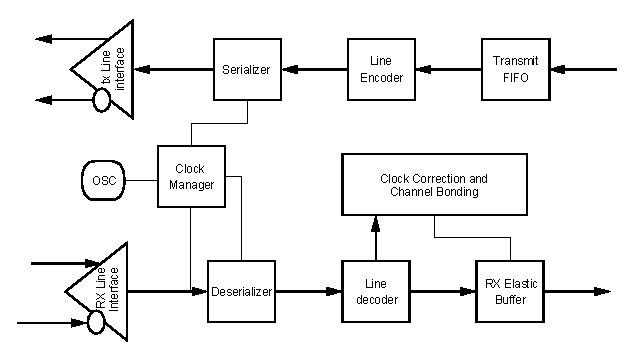
\includegraphics[width=1.0\textwidth]{ser_des}
		\caption{Arquitetura simples de um serializador e deserializador, retirada de \cite{R032}}
		\label{fig:arquiteturaSER}
	\end{center}
\end{figure}

As funções de cada bloco do diagrama do serializador apresentado passam a ser brevemente descritas:

\begin{itemize}
	\item \textbf{\textit{Transmit FIFO:}} Trata-se de uma memória FIFO que guarda os dados em paralelo antes destes serem enviados para o resto da arquitetura. No diagrama poderia também estar representa uma fonte direta de sinais em paralelo (como é o caso deste projeto).
	\item\textbf{\textit{Line Enconder:}} Este bloco trata-se de um  bloco opcional, e nem em todas as arquiteturas de serializadores/deserializadores está presente. Este bloco codifica os dados que recebe para um formato \textit{"line-friendly"} \footnote{é o termo usado pelo autor de \cite{R032}}. Trata-se de um formato que ajuda o recetor a recuperar os sinais da dados e relógio, normalmente isto envolve eliminar longas tramas de zeros ou uns, de maneira a garantir que há um equilibrio entre o número de uns e zeros numa trama.
	\item \textbf{\textit{Serializer:}} Tal como o nome indica este é um bloco que serializa os dados que recebe, ou seja, quando recebe um determinado número de dados em paralelo (x dados) a uma determinada cadência (frequência y), transforma-o num stream de dados a uma taxa de x multiplicado por y. 
	\item \textbf{\textit{TX Line Interface:}} Este bloco acaba por ser a interface final do serializador com o cabo físico, e geralmente também sofre determinados processos que permitem a melhor recuperação do sinal do lado do recetor.
\end{itemize}

Por outro lado, o deserializador tem de fazer todo o processo inverso que o bloco serializador faz. As funções de cada bloco passam a ser brevemente descritas.

\begin{itemize}
	\item \textbf{\textit{RX Line Interface:}} É a interface do deserializador com o cabo físiso. Já pode incluir alguma equalização do sinal passiva ou ativa.
	\item\textbf{\textit{Deserializer:}} Converte os dados em série que recebe a uma cadência de x multiplicado por y, em x dados paralelo a uma cadência de y.
	\item \textbf{\textit{Line Decoder:}} Descodifica os dados recebidos, se tal processo foi realizado do lado do transmissor.
	\item \textbf{\textit{RX Elastic Buffer:}} Este bloco permite o alinhamento dos dados recebidos para os repectivos limites. Tal pode ser feito automaticamente ou recorrer-se a palavras de alinhamento, trambém chamadas de "virgulas".
	\item \textbf{\textit{Clock Correction adn Channel Bonding:}} Este bloco permite que haja correcção entre as diferencças de sinais de relógio, e ainda correcção de atrasos entre diferentes canais (caso haja transmissão em vários canais). 
\end{itemize}

Existe ainda um bloco que é comum tanto ao serializador como ao deserializador que é o \textbf{\textit{Clock Manager}} que essencialmente é responsável pelos diversor processir que os sinais de relógio necessitarão: desde multiplicações de frequências, divisões e até mesmo recuperação do mesmo.

Esta arquitetura aqui apresentada acaba por apresentar os blocos essenciais para o correcto funcionamento de um serializador e deserializador, no entanto existem outras características que podem ser adicionadas: desde os diferentes tipos de codificações possiveis, até códigos detetores e corretores de erros que podem ser adicionados à arquitura.
%\begin{figure}[h!]
%	\begin{center}
%		\leavevmode
%		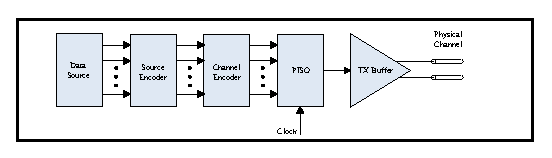
\includegraphics[width=1.0\textwidth]{ser_arq_vet}
%		\caption{Arquitetura simples de um serializador, retirada de \cite{R012}}
%		\label{fig:arquiteturaSER}
%	\end{center}
%\end{figure}



%\begin{figure}[h!]
%	\begin{center}
%		\leavevmode
%		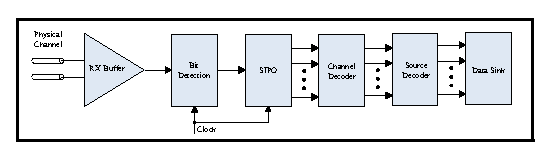
\includegraphics[width=1.0\textwidth]{des_arq_vet}
%		\caption{Arquitetura simples de um deserializador, retirada de \cite{R012}}
%		\label{fig:arquiteturaDES}
%	\end{center}
%\end{figure}

%\begin{itemize}
%	\item Chegada do sinal em paralelo ao bloco “\textit{data source}”, que corresponde à chegada dos dados em paralelo a serem posteriormente transmitidos.
%	\item Codificação da fonte (\textit{source enconding}) é bloco que se segue nesta arquitetura e inclui construção de tramas, sincronização de padrões e ainda FEC \footnote{\textit{Foward Error Correction} é uma técnica que permite o controlo de erros na transmissão de dados.}.
%	\item O bloco seguinte da arquitetura corresponde à codificação de canal, que é realizada de maneira a que o sinal a ser transmitido consiga um melhor desempenho no que toca a deteção de bits no recetor.
%	\item De seguida, o sinal codificado é enviado para o bloco PISO (\textit{parallel input - serial output)} e de onde sai um sinal em série dos dados a serem enviados.
%	\item Finalmente estes dados são enviados para o \textit{buffer} para que possam ser devidamente convertidos em sinais elétricos ou pulsos óticos para que de seguida sejam transmitidos pela camada física. 
%	\item Em alguns casos um equalizador (\textit{pre-emphasis}) para corrigir alguns erros que possam acontecer no canal em ligações de alta velocidade é utilizado. Erros podem acontecer por diversos motivos, entre os quais: a dependência da atenuação e da dispersão relativamente à frequência, interferências e ruído.
%\end{itemize}
%
%O deserializador proposto segue a mesma estrutura que o serializador fazendo, no entanto, o processo inverso.

%\subsubsection*{Considerações na implementação deste tipo de arquitetura}
%Em \cite{R012} são apontados os principais desafios na implementação deste tipo de arquitetura que passarão a ser descritos brevemente e que têm de ter sidos em conta aquando a sua implementação.




\subsubsection*{Restrições na utilização de circuitos de serializadores e deserializadores}
	
Quando se passa para a implementação de serializadores e deserializadores é necessário ter em conta algumas considerações relativamente aos circuitos utilizados. E segundo \cite{R012}, logo à partida existem grandes restrições no que toca aos circuitos utilizados nestes tipos de arquiteturas. Isto porque os sinais recebidos em paralelo são sinais digitais, contudo, quando estes sinais passam pelo canal de transmissão sofrem distorções e também lhes é adicionado ruído, o que leva a que o sinal recebido do lado do recetor seja um sinal analógico e que necessite de ser tratado como tal. A sua recuperação tem de ser então baseada na regeneração correta do sinal de relógio e também na amostragem apropriada. 
	
Ao mesmo tempo, este tipo de dispositivos são normalmente um subsistema de um sistema grande e usados em dispositivos portáteis, e como tal precisam de ter um baixo consumo de energia. Assim sendo, um dos primeiros grandes desafios desta implementação de serializador/deserializador, segundo \cite{R012}, é conseguir implementar circuitos digitais de alta velocidade e que ao mesmo tempo têm um baixo consumo de potência. Este mesmo autor apresenta duas principais técnicas utilizadas para alcançar tais objetivos que passam pela utilização de lógica CMOS que permitem a utilização a alta velocidade com baixo consumo de potência. 
	
Outro requisito crítico na implementação deste tipo de arquiteturas é também a adaptação das impedâncias características do \textit{buffer} (de transmissão e receção) com a impedância característica da linha onde é transmitido o sinal. Isto porque, caso estas não estejam adaptadas ocorrerão reflexões no lado do transmissor ou do recetor (consoante a desadaptação) que não permitem a transmissão da potência total do sinal. No entanto, este requisito requer um grande consumo de potência, pois na prática os canais de transmissão têm uma impedância muito baixa. 

\subsubsection*{Codificação dos sinais e sua importância}

\subsubsection*{PISO (\textit{Parallel input – serial output}) e SIPO (\textit{serial input – parallel output})}

Os blocos de serialização e deserialização da arquitetura têm uma grande importância no correto funcionamento de toda a arquitetura, isto porque, tal como o nome indica, estes convertem os dados em paralelo em série e vice-versa. Tal como já foi refeirdo anteriormente, o serializador recebe N dados a uma frequência de X, e transmite esses N dados a uma frequência de X*N. Por outro lado o deserializador, reduz a frequêncaia dos dados, convertendo-os em paralelo, para de seguida ser enviada para o resto da arquitetura para processamento desses mesmos dados. Por isso, é necessário tomar em atenção diversas características quanto à escolha destas arquieturas, tais como a sua latência.

O autor de \cite{R012} propõe 3 tipos de arquiteturas para este tipo de bloco que são apresentadas na imagem ~\ref{fig:PISO-SIPO} na página~\pageref{fig:PISO-SIPO} e que passam a ser descritas as suas vantagens e desvantagens.


	\begin{figure}[h!]
	\begin{center}
		\leavevmode
		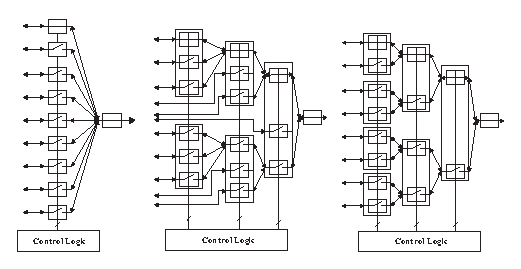
\includegraphics[width=1.0\textwidth]{SIPO_PISO_vet}
		\caption{Arquiteturas de PISO/SIPO, retirada de \cite{R012}}
		\label{fig:PISO-SIPO}
	\end{center}
\end{figure}

No circuito mais á esquerda, denominada de a) pelo autor de \cite{R012}, visualiza-se uma estrutura de um único andar, todavia esta é demasiado lenta devido às capacidades intrínsecas largas no nó de conversão. No circuito do centro, b), é representada uma topologia  heterogénea que se torna mais rápida que a apresentada em a). Já no último circuito apresentado na imagem (o da mais à direita), c), é é representada uma topologia em árvore binária que é a mais rápida segundo o autor de \cite{R012}. O autor reforça ainda a ideia de que a utilização de multiplexadores e des-mutiplexadores de 2:1 e 1:2 respectivamente são muito importantes para se obter uma arquitetura de funcionamento rápido. É de notar ainda que quando se utiliza uma arquitetura de serialização/deserialização em arvore binária, tal como o autor sugere, as portas de entrada do serializador terão dezenas de entradas, tal como as portas de saída do deserializador terão dezenas de saída, e por isso alguns pontos que necessitam de circuitos de velocidade elevada e outros que não. Para tal é necessário ter em atenção que tipo de circuitos são usados em cada etapa do serializador dada a sua necessidade de velocidade. O autor sugere a utilização de circuitos lógicos CML para as etpas que necessitam de trabalhar a altas velocidades, e CMOS para as que não necessitam de tanta velocidade.

Em situações em que as taxas de débito são muito elevadas a utilização de \textit{shift registers} torna-se também bastante eficiente para implementar um serializador/deserializador com base em \textit{shift-registers}. Neste tipo de arquitetura o serializador lê os dados para um shift register quando este se encontra com o sinal de seleccção ativa, e quando este mesmo se desliga, então os dados são enviados a alta velocidade pelo cabo fisico. No caso do serializador, os dados que chegam a alta velocidade são amostrados shiftados a cada ciclo de relógio do sinal de alta velocidade, e um sinal de relógio com uma frequência mais baixa é de seguida usado para amostrar a saída de cada registo. 


Os autores de \cite{R033} utilizam este tipo de serializadores nas suas implementações de serializadores. Vou explica-los assim muito por alto e se tiverem alguma figura alusiva vou colocar uma vez que ajuda a compreensão do funcionamento


Para que estes blocos funcionem é necessário que exista um sinal de relógio de alta frequência (à taxa de débito do canal em série) e um sinal de baixa frequência também (para a os dados em paralelo). O sinal de relógio mais alto é usado para amostrar na saída os dados provenientes do sinal em paralelo e ao mesmo tempo para amostrar os dados recebidos em série. O sinal de frequência mais baixo, é utilizado para colocar na saída os dados que são amostrados do sinal em série. Deste modo, é necessário a utilização de multiplicadores de sinal de relógio e divisores de frequências que serão de seguida mencionados.
	
\subsubsection*{Unidade de Multiplicação de Sinais de relógio (CMU – \textit{Clock Multiplier Unit})}
	
	\hspace{1.0em}O sinal de relógio de alta frequência é bastante importante na implementação de arquiteturas de serialização e deserialização de alta velocidade, isto porque este sinal é necessário tanto do lado do recetor como do transmissor, segundo a fonte \cite{R012}. Do lado do transmissor é necessário para gerar os símbolos a serem transmitidos e do lado do recetor é necessário para que a amostragem do sinal recebido possa ser bem realizada. É comum que este sinal de relógio seja então partilhado entre o recetor e o transmissor, sendo que será necessário um bloco que faça o ajuste de fase deste sinal do lado do recetor. Este é necessário por causa do atraso introduzido pelo canal, que não é conhecido à priori e também devido ao ruído introduzido no canal que tornam a fase do sinal recebido bastante crítica para o desempenho do transcetor. Esta unidade é então responsável por tal procedimento.
	
 \subsubsection*{Equalização}
	
O sinal comunicado ao longo do canal pode sofrer interferências por vários motivos, interferências essas que são críticas no que toca à receção do sinal no recetor. Como tal, existe uma necessidade de utilizar técnicas que melhorem a ligação entre os dois terminais. Segundo \cite{R012}, esta melhoria pode ser realizada através da utilização de canais de ligação de melhor qualidade. No entanto, esta opção traz custos acrescidos à ligação. 
	
Por outro lado, também pode ser utilizada uma técnica de equalização que consegue obter bons resultados sem custos acrescidos à ligação. Ainda na mesma referência são apresentadas diferentes combinações de métodos de equalização que passam a ser brevemente descritos:
	
	\begin{itemize}
		\item Linear ou não-linear
		\item Pode ser implementado do lado transmissor, ou do recetor ou ainda de ambos os lados
		\item Pode ser implementado em tempo contínuo ou discreto
		\item Pode ser adaptativo ou fixo
	\end{itemize}

	Assim sendo, existe um vasto conjunto de opções de equalização que estão diretamente relacionadas com o circuito CDR (\textit{Clock Data Recovery}), sendo que as mais importantes serão referidas mais à frente neste relatório. 

 \textbf{CDR (\textit{Clock Data Recovery})}
	
Tal como referido anteriormente, a comunicação de sinais de alta velocidade pode sofrer diversas interferências durante a sua transmissão. Contudo, segundo \cite{R012}, após a equalização do sinal estas mesmas interferências são parcialmente compensadas permitindo assim uma recuperação dos dados transmitidos.  Para fazer a correta recuperação do sinal é necessário recorrer a um circuito que recupere inicialmente o sinal de relógio transmitido do emissor para que o sinal recuperado possa ser usado para recuperação dos dados transmitidos. Uma estrutura deste tipo de circuito será descrita mais à frente neste relatório.


\subsubsection*{Restrições dos sinais de relógio de referência das arquiteturas}

\subsubsection*{Correcção do sinal de relógio}

\subsubsection*{Sinalização Física}
\subsubsection*{Pré-Enfase}
\subsubsection*{Equalização de Linha}
\subsubsection*{Criação de Protocolos}

%\section{Serializador e Deserializador disponíveis na FPGA}
%
%As FPGA de série 7 da XILINX têm disponíveis transcetores capazes de comunicação em série de alta velocidade, tal como é necessário neste projeto. Em específico, na FPGA XILINX VC7203 Virtex-7 estão disponíveis transcetores GTX que permitem uma velocidade de 10 Gb/s e que são os mais adequados para conexão à fibra ótica. Noutros modelos existem outros transcetores, como por exemplo GTZ (que permite até 28 Gb/s), GTH (que permite débitos até 13,1 Gb/s) e GTP (com débitos até 6,6 Gb/s). No entanto apenas serão abordados os transcetores GTX, visto que são os mais adequados para este tipo de comunicações.
%
%\begin{figure}[h!]
%	\begin{center}
%		\leavevmode
%		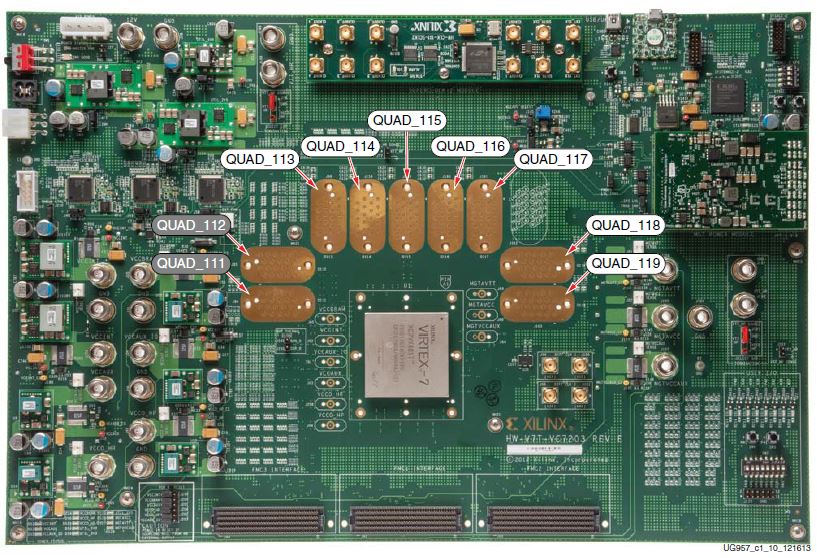
\includegraphics[width=1.0\textwidth]{gtxLOCA}
%		\caption{Identificação dos transcetores GTX na FPGA VC7203 Virtex-7, retirada de \cite{R008}}
%		\label{fig:GTXlocalização}
%	\end{center}
%\end{figure}
%
%Na figura~\ref{fig:GTXlocalização} na página~\pageref{fig:GTXlocalização} é possível visualizar a FPGA a ser utilizada no projeto e visualiza-se ainda assinaladas as entradas GTX (QUAD\_111, QUAD\_112, QUAD\_113, QUAD\_114, QUAD\_115, QUAD\_116, QUAD\_117, QUAD\_118 e QUAD\_119). 
%Os transcetores baseiam-se na seguinte arquitetura, segundo \cite{R010}:
%\begin{itemize}
%	\item \textbf{PMA (\textit{Physical Medium Attachment Sublayer})} que inclui:
%	\begin{itemize}
%		\item suporte de taxas de débito até 12,5 Gb/s
%		\item uma PLL por canal para melhor flexibilidade do sinal de relógio
%		\item uma interface que faz a conversão de série para paralelo e de paralelo para série (PISO e SIPO)
%		\item uma PLL (\textit{Phase-Locked Loop})
%		\item Equalizador de decisão com feedback (DFE)
%		\item CDR (\textit{clock data recovery})
%		\item Bloco de pré-ênfase e equalização
%		\item Saída do transmissor programável
%	\end{itemize}
%	\item \textbf{PCS (\textit{Physical Coding Sublayer}) que inclui:}
%	\begin{itemize}
%		\item \textit{Datapath} de 2 e 4 byte internos para suportar diferentes taxas de débitos
%		\item Codificação e descodificação 8B/10B
%		\item Deteção de vírgula e alinhamento de palavra
%		\item PRBS (\textit{Pseudo Random Bit Sequence}) gerador e verificador
%		\item FIFO para correção do sinal de relógio e ligação do canal
%		\item Lógica que processa os dados em paralelo reconfigurável
%		\item Este bloco trabalha com taxas de débitos de informação mais baixas.
%	\end{itemize}
%\end{itemize}
%
%É possível visualizar um diagrama geral da arquitetura dos transcetores GTX disponíveis na FPGA na figura~\ref{fig:GTXarquitetura} na página~\pageref{fig:GTXarquitetura}.
%
%\begin{figure}[h!]
%	\begin{center}
%		\leavevmode
%		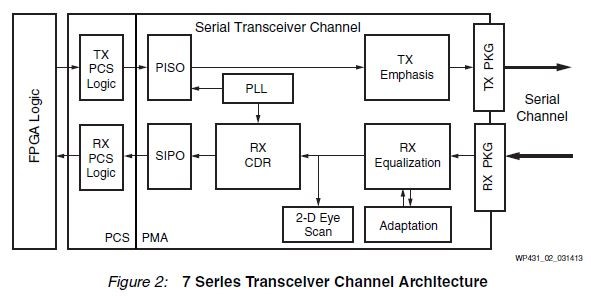
\includegraphics[width=1.0\textwidth]{gtxAqr}
%		\caption{Arquitetura geral dos transcetores GTX, retirada de \cite{R010}}
%		\label{fig:GTXarquitetura}
%	\end{center}
%\end{figure}
%
%O transmissor e o recetor passam a ser descritos mais detalhadamente de seguida.
%
%\subsubsection{Transmissor}
%Cada transcetor GTX inclui um transmissor independente que consiste num módulo PCS e um modulo PMA, tal como referido anteriormente. A figura~\ref{fig:gtx_tx} na página~\pageref{fig:gtx_tx} representa o diagrama de blocos do transmissor.
%\begin{figure}[h!]
%	\begin{center}
%		\leavevmode
%		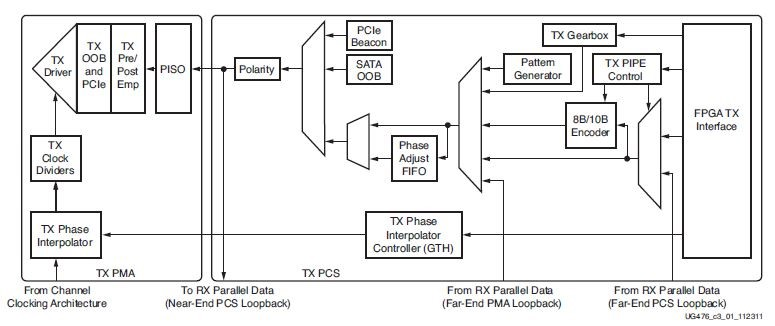
\includegraphics[width=1.0\textwidth]{gtx_tx}
%		\caption{Diagrama de blocos de um transmissor GTX, retirada de \cite{R011}}
%		\label{fig:gtx_tx}
%	\end{center}
%\end{figure}
%
%Os dados provenientes da FPGA, cujo formato é em paralelo, passam para a interface transmissora, de seguida para os módulos PCS e PMA e, por fim, para a saída pelo driver do transmissor a alta velocidade. 
%
%O transmissor contém os seguintes blocos principais, cujas funcionalidades passam a ser brevemente resumidas, segundo \cite{R010}:
%\begin{enumerate}
%	
%
%	\item \textbf{Interface transmissora da FPGA}
%	
%	\hspace{1.0em}Esta interface serve como porta de comunicação entre a FPGA e o datapath do transmissor. Esta comunicação é feita através da escrita de dados na porta TXDATA na transição de 0 para 1 do sinal de relógio TXUSRCLK2.
%	
%	\hspace{1.0em}O tamanho do sinal a ser transmitido pode ser configurado para 2, 4 ou 8 bytes. Na realidade este tamanho é definido por TX\_DATA\_WIDTH e TX\_INT\_DATAWIDTH e ainda por TX8B19BEN, e o tamanho interno destes sinais pode ser 16, 20, 32, 40, 64 e 80 bits. A tabela~\ref{table:dataTXDATA} na página~\pageref{table:dataTXDATA} demonstra como esses tamanhos são configurados através das entradas referidas.
%	
%% Please add the following required packages to your document preamble:
%% \usepackage{multirow}
%\begin{table}[]
%	\centering
%	\begin{tabular}{|c|c|c|c|c|}
%		\hline
%		\textbf{TX8B10BEN} & \textbf{TX\_DATA\_WIDTH} & \textbf{TX\_INT\_DATAWIDTH} & \textbf{\begin{tabular}[c]{@{}c@{}}Tamanho na interface \\ da FPGA (bits)\end{tabular}} & \textbf{\begin{tabular}[c]{@{}c@{}}Tamanho interno \\ dos dados (bits)\end{tabular}} \\ \hline
%		\multirow{4}{*}{1} & 20                       & 0                           & 16                                                                                      & 20                                                                                   \\ \cline{2-5} 
%		& 40                       & 0                           & 32                                                                                      & 20                                                                                   \\ \cline{2-5} 
%		& 40                       & 1                           & 32                                                                                      & 40                                                                                   \\ \cline{2-5} 
%		& 80                       & 1                           & 64                                                                                      & 40                                                                                   \\ \hline
%		\multirow{8}{*}{0} & 16                       & 0                           & 16                                                                                      & 16                                                                                   \\ \cline{2-5} 
%		& 20                       & 0                           & 20                                                                                      & 20                                                                                   \\ \cline{2-5} 
%		& 32                       & 0                           & 32                                                                                      & 16                                                                                   \\ \cline{2-5} 
%		& 32                       & 1                           & 32                                                                                      & 32                                                                                   \\ \cline{2-5} 
%		& 40                       & 0                           & 40                                                                                      & 20                                                                                   \\ \cline{2-5} 
%		& 40                       & 1                           & 40                                                                                      & 40                                                                                   \\ \cline{2-5} 
%		& 64                       & 1                           & 64                                                                                      & 32                                                                                   \\ \cline{2-5} 
%		& 80                       & 1                           & 80                                                                                      & 40                                                                                   \\ \hline
%	\end{tabular}
%	\caption{Configuração do tamanho dos dados de TXDATA, adaptada de \cite{R011}}
%	\label{table:dataTXDATA}
%\end{table}
%
%	\hspace{1.0em}Quando o codificador 8B/10B está ativo, então TX\_DATA\_WIDTH deve estar configurado para 20, 40 ou 80 bits e nesta situação, a interface do transmissor com a FPGA apenas utiliza os dados provenientes da porta TX\_DATA\_WIDTH. Quando o mesmo está desativo, então TX\_DATA\_WIDTH pode estar configurado para 16,20,32,40,64 ou 80 bits.
%
%	\hspace{1.0em}O sinal TX\_INT\_DATAWITH é um atributo que configura a ativação do datapath de 2 e 4 bytes disponível internamente no transcetor.
%
%	\hspace{1.0em}Para além do sinal de relógio TXUSRCLK2, que é o sinal de relógio principal para a sincronização dos sinais que chegam ao transmissor, existe um segundo sinal de relógio paralelo que é usado internamente para operações lógicas a realizar no módulo PCS. Este segundo sinal de relógio, TXUSRCLK, irá depender do tamanho interno dos dados usado no datapath e da taxa de transmissão do transmissor GTX. É possível calcular esta mesma taxa através da divisão entre a taxa de transmissão da linha e do tamanho interno dos dados utilizado no datapath. Para além disso, estes dois sinais de relógio têm uma relação fixa que determina os seus valores que depende dos valores presentes em TX\_DATA\_WIDTH e TX\_INT\_DATAWIDTH. Essas relações estão apresentadas na tabela~\ref{table:freqTXgtx} na página~\pageref{table:freqTXgtx}:
%
%\begin{table}[]
%	\centering
%	\begin{tabular}{|c|c|c|c|}
%		\hline
%		\textbf{\begin{tabular}[c]{@{}c@{}}Tamanho na \\ interface da\\  FPGA (byte)\end{tabular}} & \textbf{TX\_DATA\_WIDTH} & \textbf{TX\_INT\_DATAWIDTH} & \textbf{Frequência de TXUSRCLK2} \\ \hline
%		2                                                                                          & 16, 20                   & 0                           & f(TXUSRCLK2) = f(TXUSRCLK)       \\ \hline
%		4                                                                                          & 32, 40                   & 0                           & f(TXUSRCLK2) = f(TXUSRCLK) / 2   \\ \hline
%		4                                                                                          & 32, 40                   & 1                           & f(TXUSRCLK2) = f(TXUSRCLK)       \\ \hline
%		8                                                                                          & 64, 80                   & 1                           & f(TXUSRCLK2) = f(TXUSRCLK) / 2   \\ \hline
%	\end{tabular}
%	\caption{Configuração da frequência de TXUSRCLK2, adaptada de \cite{R011}}
%	\label{table:freqTXgtx}
%\end{table}
%
%	\hspace{1.0em}Assim sendo, é possível fazer uso dos transcetores disponíveis na FPGA, utilizando um tamanho adequado de dados para a transmissão, tendo em conta as configurações necessárias e disponíveis para tal, tal como descrito anteriormente. Por outras palavras, utilizando tamanhos de entradas devidamente apropriados, será fácil enviar os dados recebidos e descodificados do HDMI através destes transcetores, que pode vir a ser útil numa fase inicial do projeto.
%
%	\item \textbf{Codificador 8B/10B do transmissor}
%	
%	\hspace{1.0em}Esta é a codificação utilizada no sinal para de seguida fazê-lo enviar pelas portas de alta velocidade, e é uma codificação \textit{standard} que troca dois bits por byte para alcançar um equilíbrio e obter uma disparidade limitada para que a recuperação de relógio seja razoável. O transmissor possui um \textit{datapath} específico para fazer este tipo de codificação e ao mesmo tempo poupar recursos da FPGA apesar de aumentar a latência no caminho do transmissor.
%	
%	\hspace{1.0em}A ativação ou não deste bloco é representada no sinal TX8B10BEN. Quando está ativo, o sinal passado na interface do transmissor com a FPGA por TXDATA é codificado antes de ser enviado pelas saídas de alta velocidade, caso contrário, tal não acontece e o sinal é enviado tal como é transmitido. 
%	
%	\item \textbf{\textit{Gearbox} do transmissor}
%	
%	\hspace{1.0em}Este bloco suporta a codificação do sinal 64B/66B e 64B/67B, uma vez que este tipo de codificação é utilizada em alguns protocolos de comunicação de alta velocidade. Esta utilização permite reduzir a sobrecarga da codificação 8B/10B e ao mesmo tempo reter os benefícios de um esquema de codificação. Este bloco suporta interfaces de 2, 4 ou 8 bytes e a codificação dos dados é feita na lógica da FPGA. 
%	
%	\item \textbf{\textit{Buffer} do transmissor}
%	
%	\hspace{1.0em}O transmissor GTX tem disponível também um buffer e um bloco de alinhamento de fase no seu circuito para que possa sincronizar os diferentes domínios dos sinais de relógio. Isto acontece porque internamente o transmissor tem dois sinais de relógios paralelos: o sinal do domínio PMA (XCLK) e o sinal de relógio TXUSRCLK. No entanto, quando a transmissão de dados entre estes dois domínios é realizada é necessário que os sinais estejam sincronizados e as diferenças de fase resolvidas. Como tal, será necessário a utilização deste bloco para se poder realizar a sincronização entre os sinais.
%	
%	\hspace{1.0em}O circuito de alinhamento da fase é utilizado para resolver a diferença entre as fases dos sinais quando o buffer não está ativo. Mas pelo menos um dos blocos deve ser sempre utilizado. 
%	
%	\hspace{1.0em}A utilização do \textit{buffer} é mais fácil e é sempre recomendada a sua utilização, enquanto que o bloco de alinhamento de fase é um bloco mais complexo no que toca a lógica e que requer restrições adicionais nas fontes dos sinais de relógio. Por outro lado, o buffer não deve ser utilizado quando a latência é uma questão importante do circuito, uma vez que o bloco de alinhamento de fase consegue alcançar menor latência. 
%	
%	\item \textbf{Gerador de padrões do transmissor} 
%	
%	\hspace{1.0em}A geração de sequência pseudoaleatórias é bastante utilizada em sistemas de telecomunicações para testar a integridade do sinal de ligações de grande velocidade. Apesar de estas mesmas sequências parecerem aleatórias à primeira vista, na realidade apresentam determinadas características que são utilizadas para medir a qualidade da ligação. Este bloco do transmissor é responsável por esta ação. 
%	
%	\item \textbf{Controlo de polaridade do transmissor} 
%	
%	\hspace{1.0em}Este bloco é responsável por inverter os dados em paralelo antes da sua serialização e transmissão para compensar a inversão de polaridade no par diferencial, isto porque tal pode levar a uma inversão de polarização dos dados transmitidos pelo GTX quando TXN e TXP são acidentalmente trocados na PCB. 
%	
%	\item \textbf{Controlo do sinal de relógio de saída do transmissor}
%	
%	\hspace{1.0em}Este bloco é responsável pelo controlo da divisão do sinal de relógio em série e pelo controlo da divisão e seleção do sinal de relógio em paralelo.
%	
%	\hspace{1.0em}No que toca à divisão do sinal de relógio em série, cada módulo PMA do transmissor possui um divisor D que divide o sinal de relógio da PLL para suportar taxas de transmissão mais baixas. Este divisor pode ser definido estaticamente para aplicações com uma taxa de transmissão fixa, mas também pode ser utilizado para ligações onde a taxa de transmissão pode variar e como tal D varia com essa mesma variação. Este bloco é responsável por esta divisão do sinal de relógio em série. 
%	
%	\hspace{1.0em}Quanto à divisão e seleção do sinal de relógio paralelo, o sinal de relógio em paralelo que sai deste bloco de controlo de divisão de relógio pode ser utlizado como o relógio de fabrico lógico, dependendo das linhas de transmissão requisitadas. Este bloco controla também essa mesma divisão e seleção.
%	
%	\item \textbf{Driver reconfigurável do transmissor}
%	
%	\hspace{1.0em}É um \textit{buffer} de saída diferencial de alta velocidade que possui características para maximizar a integridade do sinal, tal como controlo diferencial de tensão, pré-ênfase e resistências de terminação calibradas.
%	
%	\item \textbf{Suporte de deteção de recetor para arquiteturas \textit{PCI Express}}
%	
%	\hspace{1.0em}As especificações das arquiteturas PCI Express incluem características que permitem detetar a presença do recetor para uma determinada ligação. Este bloco é responsável por esta mesma deteção.	
%\end{enumerate}
%
%\subsubsection{Recetor}
%
%Cada transcetor possui um recetor independente, cujo diagrama de blocos está representado na figura~\ref{fig:gtx_rx} na página~\pageref{fig:gtx_rx}. Mais uma vez, o recetor possui dois módulos principais: PCS e PMA. 
%
%O sinal de alta velocidade em série chega ao RX ao modulo PMA, passa por PCS e, por fim, passa para a lógica da FPGA pela interface com a mesma.
%
%\begin{figure}[h!]
%	\begin{center}
%		\leavevmode
%		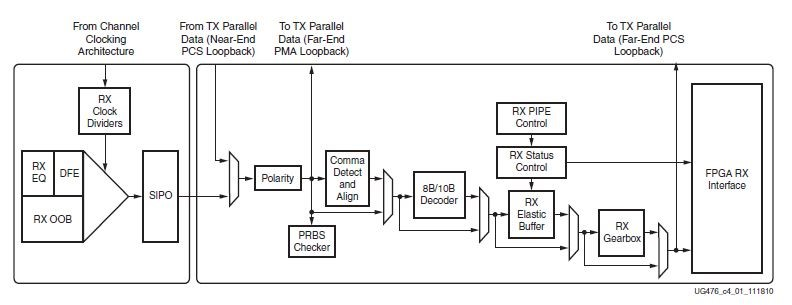
\includegraphics[width=1.0\textwidth]{gtx_rx}
%		\caption{Diagrama de blocos de um recetor GTX, retirada de \cite{R011}}
%		\label{fig:gtx_rx}
%	\end{center}
%\end{figure}
%
%É possível dividir o recetor GTX nos seguintes principais blocos que passam brevemente a ser descritos:
%
%\begin{enumerate}
%	\item \textbf{\textit{Front End} Analógico do recetor}
%	
%	\hspace{1.0em}É um buffer diferencial de entrada de modo de corrente de alta velocidade que possui determinadas características tais como: reconfiguração de tensão de terminação do recetor e calibração das resistências de terminação.
%	
%	\item \textbf{Equalizador do recetor}
%	
%	\hspace{1.0em}Ao longo da transmissão, diversos erros podem acontecer nos dados transmitidos e, como tal, são necessários filtros que permitam ou que pelo menos ajudem a realizar a recuperação do sinal recebido corretamente. Os transcetores GTX disponibilizam filtros adaptativos para tal recuperação: LPM que está otimizado para canais com poucas perdas e ainda DFE para canais com perdas maiores. As arquiteturas apresentadas de seguida foram arquiteturas brevemente abordadas anteriormente dentro deste capítulo que estão referidas em \cite{R012}.
%	
%	\hspace{1.0em}Na figura~\ref{fig:eq_LPM} na página~\pageref{fig:eq_LPM} encontra-se o diagrama de blocos do equalizador LPM. Este modo é recomendado para aplicações com débitos até 11,2 Gb/s de curto alcance, com perdas de canal até 12 dB à frequência de Nyquist.
%	
%	\begin{figure}[h!]
%		\begin{center}
%			\leavevmode
%			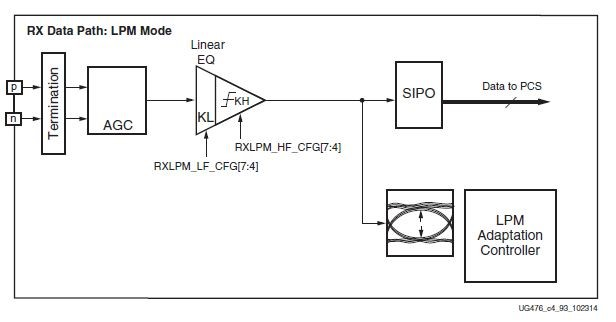
\includegraphics[width=1.0\textwidth]{equalizador_LPM}
%			\caption{Equalizador em modo LPM, retirada de \cite{R011}}
%			\label{fig:eq_LPM}
%		\end{center}
%	\end{figure}
%
%	\hspace{1.0em}Na figura~\ref{fig:eq_DFE} na página~\pageref{fig:eq_DFE} é possível visualizar o diagrama de blocos utilizado para o equalizador DFE (Decision Feedback Equalizer). Este é um filtro que utiliza a realimentação de símbolos detetados para produzir uma estimação da saída do canal. O DFE é alimentado com os símbolos já detetados e produz uma saída que é a combinação da saída do equalizador linear com estes mesmo símbolos já detetados.  
%
%	\begin{figure}[h!]
%	\begin{center}
%		\leavevmode
%		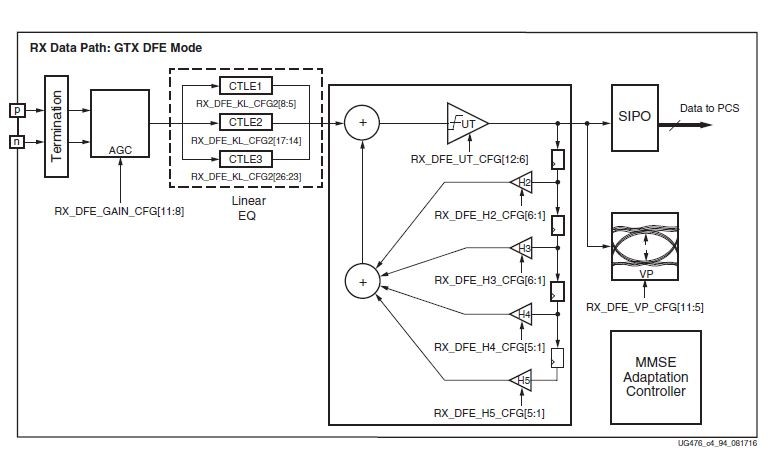
\includegraphics[width=1.0\textwidth]{equalizador_DFE}
%		\caption{Equalizador em modo DFE, retirada de \cite{R011}}
%		\label{fig:eq_DFE}
%	\end{center}
%	\end{figure}	
%
%	\hspace{1.0em}Este equalizador é utilizado para ligações de média distância cujas perdas do canal rondam os 8 dB ou mais à frequência de Nyquist. 
%	
%	\hspace{1.0em}\textbf{Vantagens da utilização deste tipo de equalizador:}
%	\begin{itemize}
%		\item Efetua a equalização sem amplificação do ruído ou interferência
%		\item Pode também fazer correções de reflexões causadas pelas descontinuidades do canal 
%		\item É vantajosa a sua utilização quando as interferências são preocupantes 
%	\end{itemize}
%	
%	\hspace{1.0em}\textbf{Cuidados a ter na utilização deste tipo de equalizador:}
%	\begin{itemize}
%		\item Este tipo de equalização deve ser cuidadosa quando não existe codificação de dados, uma vez que pode levar à não equalização ideal do sinal recebido (pois o filtro pode não se auto adaptar aos dados recebidos).
%	\end{itemize}
%
%	\hspace{1.0em}Visto que neste projeto se pretende realizar comunicações de média/longa distância, deve ser utilizado o equalizador DFE para obter uma boa equalização do sinal recebido. 
%	
%	\item \textbf{CDR (\textit{Clock Data Recovery}) do recetor}
%	
%	\hspace{1.0em}O circuito de CDR faz a recuperação do relógio dos dados recebidos em série. Na figura~\ref{fig:cdr} na página~\pageref{fig:cdr} é possível encontrar a arquitetura deste mesmo circuito. Este circuito foi também já brevemente referido no subcapítulo anterior que refere as considerações a tomar quando se implementam arquiteturas de serialização e deserialização, e passa de seguida a ser descrito.
%	
%	\begin{figure}[h!]
%		\begin{center}
%			\leavevmode
%			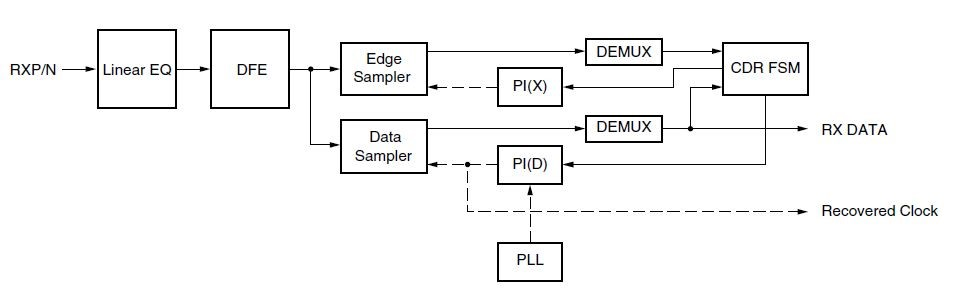
\includegraphics[width=1.0\textwidth]{CDR}
%			\caption{Detalhes do circuito CDR (\textit{Clock data recovery}), retirada de \cite{R011}}
%			\label{fig:cdr}
%		\end{center}
%	\end{figure}
%
%	\hspace{1.0em}A tracejado encontra-se o caminho feito pelo sinal de relógio até à sua recuperação. 
%	Os dados recebidos passam pelo equalizador e de seguida são capturados por um “data sampler” e um “edge sampler”. O “edge sampler” captura a fase do sinal recebido em série quando este está na sua região de transição, enquanto que o “data sampler” captura a fase do mesmo sinal a meio do olho dos dados. Estas duas fases são de seguida enviadas para a máquina de estados do CDR para que esta consiga determinar a fase dos sinais que chegam e ao mesmo tempo controlar os interpoladores de fase (PIs).
%	
%	\item \textbf{Controlo do sinal de relógio de saída} 
%	
%	Tal como no transmissor, o bloco de divisão de sinal de relógio tem dois principais componentes: controlo da divisão do sinal de relógio em série e ainda controlo e seleção da divisão do sinal relógio em paralelo. As suas funções são iguais à do transmissor.
%	
%	\item \textbf{Análise de Margem do Recetor}
%	
%	\hspace{1.0em}Com o aumento das taxas de débito da transmissão e também da atenuação os equalizadores dos recetores têm mais capacidade de superar a atenuação do canal. Contudo, isto traz um novo desafio, pois nestes casos, a qualidade da ligação não pode ser medida através da abertura do olho no diagrama de olho resultante. 
%	
%	\hspace{1.0em}Para taxas de transmissão muito altas pode acontecer que o diagrama de olho do sinal recebido possa parecer completamente fechado, apesar de que após a equalização esteja aberto. Como tal, esta medida de qualificação da qualidade da ligação realizada pode então ter de ser reavaliada.
%	
%	\hspace{1.0em}Assim sendo, os transmissores GTX possuem um mecanismo que permite medir e visualizar a margem do diagrama de olho recebido após equalização. Também existem modos que permitem determinar e diagnosticar os efeitos das configurações de equalização.
%	
%	\hspace{1.0em}Este mecanismo permite que uma correta avaliação da qualidade do canal e para além disso, pode ser feita enquanto os dados estão a ser recebidos, devido ao seu mecanismo que assim o permite, não exigindo nenhuma alteração às configurações do recetor e nem nenhuma lógica extra da FPGA. 
%	
%	\item \textbf{Controlo da polarização do recetor}
%	
%	\hspace{1.0em}Tal como foi mencionado aquando a referência da funcionalidade deste mesmo bloco no transmissor, os sinais RXN e RXP podem ser trocados acidentalmente na PCB e como tal os dados diferencias recebidos pelo recetor estão invertidos. Este bloco é responsável pela inversão dos bytes em paralelo no módulo PCS antes da deserialização do sinal (SIPO) para compensar a polarização inversa do par diferencial.
%	
%	\item \textbf{Verificador de Padrões do recetor}
%	
%	\hspace{1.0em}Este bloco é responsável pela verificação de determinados padrões PSBR e faz esta mesma verificação antes do alinhamento das palavras ou descodificação. Tal como descrito aquando a referência ao gerador destes mesmos padrões no transmissor, estes servem para verificar a integridade do sinal na ligação.
%	
%	\item \textbf{Alinhamento de \textit{Byte} e palavras do recetor}
%	
%	\hspace{1.0em}Os dados em série que chegam ao recetor devem ser alinhados com limitações de símbolos antes de poderem ser utilizados como dados em paralelo. Assim sendo, o transmissor envia sequências reconhecíveis (normalmente são chamadas de vírgulas) e o recetor procura essa mesma sequência nos dados recebido. Quando a encontra move-a para os limites das palavras para que as palavras em paralelo recebidas sejam iguais às palavras enviadas pelo transmissor. Para ativar a utilização deste bloco o sinal de entrada RXCOMMADETEN deve ser verdadeiro, mas caso a latência seja um parâmetro critico do circuito então este bloco não deve estar ativo. 
%	
%	\hspace{1.0em}Para definir a sequência que o bloco de alinhamento deve procurar (a vírgula) nos dados que chegam em série ao recetor, então deve-se definir as entradas ALIGB\_MCOMMA\_VALUE, ALIGN\_PCOMMA\_VALUE e ALIGN\_COMMA\_ENABLE. Os tamanhos destas sequências dependerão dos valores em RX\_DATA\_WIDTH, que será explicado mais à frente neste relatório.
%	
%	\begin{figure}[h!]
%		\begin{center}
%			\leavevmode
%			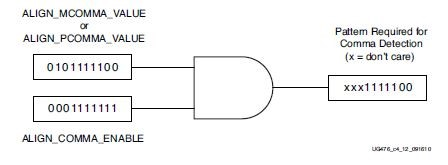
\includegraphics[width=0.7\textwidth]{commaObtain1}
%			\caption{Mecanismo de obtenção da “vírgula”, retirado de \cite{R011}}
%			\label{fig:comma1}
%		\end{center}
%	\end{figure}
%	
%	\hspace{1.0em}A figura~\ref{fig:comma1} na página~\pageref{fig:comma1} ilustra o mecanismo utlizado para obter a sequência de procura dos dados recebidos no recetor quando ALIGN\_COMMA\_DOUBLE é falso. Quando este mesmo sinal é verdadeiro faz-se então uma extensão do sinal ALIGN\_MCOMMA\_VALUE e do sinal ALIGN\_PCOMMA\_VALUE, tal como está representado na figura~\ref{fig:comma2} na página \pageref{fig:comma2}.
%	
%		\begin{figure}[h!]
%		\begin{center}
%			\leavevmode
%			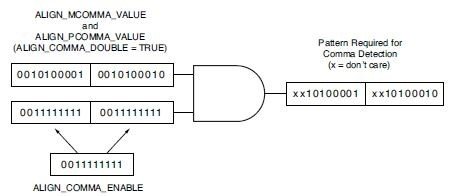
\includegraphics[width=0.7\textwidth]{commaObtain2}
%			\caption{Mecanismo de obtenção da “vírgula” quando ALIGN\_COMMA\_DOUBLE=1, retirado de \cite{R011}}
%			\label{fig:comma2}
%		\end{center}
%	\end{figure}
%	
%	\hspace{1.0em}Quando este mesmo sinal está ativo os sinais de entrada ALIGN\_MCOMMA\_VALUE e ALIGN\_PCOMMA\_VALUE são combinados e o bloco procura por duas sequências de uma vez nos mesmos dados recebidos. Para ativar o alinhamento de palavras da sequência MCOMMA o sinal RXMCOMMAALIGNEN deve estar ativo, enquanto que para ativar o alinhamento da palavra PCOMMA o sinal RXPCOMMAALIGNEN deve estar ativo. Quando ambas estão ativas então o alinhamento é realizado com qualquer padrão.
%	
%	\hspace{1.0em}É necessário ter em atenção que em aplicações cuja taxa de débito é superior a 5 Gb/s e que têm demasiado ruído, pode acontecer por vezes um falso alinhamento de palavras que leva à ativação do sinal. Isto indica que as palavras estão alinhadas sem realmente haver dados válidos presentes nelas. Assim sendo, neste tipo de sistemas é necessária a presença de um sistema que faça a verificação da validade destes dados alinhados para prevenir casos como estes.
%	
%	\hspace{1.0em}Deste modo, com esta característica do recetor GTX da FPGA o alinhamento de palavras torna-se simplificado.
%	
%	\item \textbf{Descodificador 8B/10B do recetor}
%	
%	\hspace{1.0em}Se os sinais estiverem codificados segundo 8B/10B então devem ser descodificados segundo esta norma também. Desta forma, o recetor possui um bloco responsável pela descodificação 8B/10B no recetor sem que gaste recursos adicionais à FPGA. Este mesmo bloco pode não estar ativo caso o sinal tenha codificação 8B/10B.
%	
%	\item \textbf{\textit{Buffer} do recetor}
%	
%	\hspace{1.0em}Tal como no transmissor o \textit{buffer} é utilizado para possibilitar a sincronização entre o domínio do sinal de relógio do PMA em paralelo e o sinal de relógio RXUSRCLK. Isto porque, para ser possível a transmissão de dados entre os dois domínios a taxa do domínio PMA dever ser suficientemente parecida com a taxa de RXUSRCLK e todas as diferenças de fases entre as mesmas devem estar resolvidas. Este é, então, o bloco responsável por estes ajustes que devem ser feitos. Alternativamente a este buffer pode ser utilizado o circuito de alinhamento de fase, tal como foi referido anteriormente. No entanto, existem algumas vantagens e desvantagens de utilização destas duas opções.
%	
%	\hspace{1.0em}A utilização do \textit{buffer} torna-se mais fácil em termos de operação, enquanto que o circuito de alinhamento exige lógica extra e restrições adicionais relativamente às fontes do sinal de relógio, tal como acontecia para o transmissor. Quanto à utilização de sinais de relógio o buffer pode usar tanto o sinal de relógio recuperado como o sinal de relógio local, enquanto que o circuito de alinhamento de fase apenas pode utilizar o sinal de relógio recuperado pelo recetor. Relativamente aos tempos de estabilização a utilização do buffer não necessita de começar a funcionar imediatamente após a sua inicialização, enquanto que o circuito de alinhamento do sinal necessita de esperar pela estabilização de todos os sinais de relógio antes de conseguir realizar qualquer alinhamento de fase ou atraso. Em contrapartida, o buffer tem uma latência maior do que o circuito de alinhamento de fase, apesar de essa mesma latência depender também de algumas características do mesmo, como por exemplo a correção do sinal de relógio ou a ligação entre os canais do recetor.
%	
%	\item \textbf{Correção do Sinal de relógio do recetor }
%	
%	\hspace{1.0em}Este bloco é responsável por evitar o overflow do buffer, isto porque o buffer faz a ponte de ligação entre dois domínios de sinal de relógio que apesar de serem muito idênticos nunca serão iguais. Como tal, haverá sempre uma ligeira diferença de fase entre os dois sinais causando acumulação que podem levar a um overflow ou underflow a não ser que seja corrigido. 
%	
%	\hspace{1.0em}Para fazer esta correção, cada transmissor envia periodicamente um ou mais caracteres especiais que permitem que o recetor os elimine ou replique no buffer consoante a necessidade. Através da remoção desses caracteres quando o buffer está muito cheio e a sua replicação quando o \textit{buffer} está vazio o recetor previne o \textit{oveflow} ou \textit{underflow}. 
%	
%	\item \textbf{\textbf{Ligação de canais do recetor}}
%	
%	\hspace{1.0em}Este bloco é responsável por fazer chegar todos os canais ao mesmo tempo ao recetor. Isto acontece porque existem protocolos que combinam múltiplos transcetores para criar um único canal de saída de alta velocidade. A diferença entre os tamanhos dos sinais de cada transcetor pode fazer com que os sinais sejam enviados todos ao mesmo tempo, mas que cheguem a tempos diferentes ao recetor. Este bloco é responsável por eliminar este efeito através do uso de um buffer como um bloco cuja latência é variável. 
%	
%	\hspace{1.0em}Os transmissores GTX enviam um caracter que identifica a ligação entre canais (ou uma sequência de caracteres) simultaneamente. Quando este é recebido o recetor é capaz de determinar a diferença entre cada canal e ajustar a latência do buffer para que os dados cheguem todos ao mesmo tempo a interface com o utilizador. 
%	
%	\item \textbf{\textit{Gearbox} do receto}r
%	
%	\hspace{1.0em}Este bloco é similar ao bloco gearbox do transmissor referido anteriormente neste relatório.
%	
%	\item \textbf{Interface do recetor com FPGA}
%	
%	\hspace{1.0em}Este bloco é responsável pela comunicação entre o recetor e a FPGA, ou seja, a FPGA consegue ler os dados recebidos no recetor através da leitura do sinal RXDATA na transição de 0 para 1 do sinal de relógio RXUSRCLK2. O tamanho desta porta pode ser configurado para 2, 4 ou 8 bytes, mas a largura real da porta depende de RX\_DATA\_WIDTH, RX\_DATAWIDTH e RX8B10BEN, tal como no transmissor. Assim, os tamanhos dos dados das portas pode ser 16, 20, 32, 40, 64 ou 80 bits.
%	
%	\hspace{1.0em}O recetor dos transcetores GTX contém datapaths internos de 2 e 4 bytes que são configuráveis através do atributo RX\_INT\_DATAWIDTH. A largura dos sinais na interface da FPGA é configurável através do sinal RX\_DATA\_WIDTH que deve ser 20, 40 ou 80 bits no caso de o descodificador 8B/10B estar ativo. Neste caso, a interface do recetor com a FPGA apenas usa as portas RXDATA. Quando o descodificador 8B/10B não é utilizado então RX\_DATA\_WIDTH pode ser configurado para outro qualquer valor disponível. O valor do tamanho dos sinais para as diferentes configurações no recetor está disponível na tabela\ref{table:dataRXDATA} na página~\pageref{table:dataRXDATA}.
%	
%	
%% Please add the following required packages to your document preamble:
%% \usepackage{multirow}
%\begin{table}[]
%	\centering
%	\begin{tabular}{|c|c|c|c|c|}
%		\hline
%		\textbf{RX8B10BEN} & \textbf{RX\_DATA\_WIDTH} & \textbf{RX\_INT\_DATAWIDTH} & \textbf{\begin{tabular}[c]{@{}c@{}}Tamanho na \\ interface da \\ FPGA (bits)\end{tabular}} & \textbf{\begin{tabular}[c]{@{}c@{}}Tamanho \\ interno dos \\ dados (bits)\end{tabular}} \\ \hline
%		\multirow{4}{*}{1} & 20                       & 0                           & 16                                                                                         & 20                                                                                      \\ \cline{2-5} 
%		& 40                       & 0                           & 32                                                                                         & 20                                                                                      \\ \cline{2-5} 
%		& 40                       & 1                           & 32                                                                                         & 40                                                                                      \\ \cline{2-5} 
%		& 80                       & 1                           & 64                                                                                         & 40                                                                                      \\ \hline
%		\multirow{8}{*}{0} & 16                       & 0                           & 16                                                                                         & 16                                                                                      \\ \cline{2-5} 
%		& 20                       & 0                           & 20                                                                                         & 20                                                                                      \\ \cline{2-5} 
%		& 32                       & 0                           & 32                                                                                         & 16                                                                                      \\ \cline{2-5} 
%		& 32                       & 1                           & 32                                                                                         & 32                                                                                      \\ \cline{2-5} 
%		& 40                       & 0                           & 40                                                                                         & 20                                                                                      \\ \cline{2-5} 
%		& 40                       & 1                           & 40                                                                                         & 40                                                                                      \\ \cline{2-5} 
%		& 64                       & 1                           & 64                                                                                         & 32                                                                                      \\ \cline{2-5} 
%		& 80                       & 1                           & 80                                                                                         & 40                                                                                      \\ \hline
%	\end{tabular}
%	\caption{Configuração do tamanho dos dados de RXDATA, adaptada de \cite{R011}}
%	\label{table:dataRXDATA}
%\end{table}
%	\hspace{1.0em}A interface do recetor com a FPGA inclui dois sinais de relógio em paralelo: RXUSRCLK e RXUSRCLK2. A taxa de débito do sinal de relógio paralelo RXUSRCLK2 na interface é determinada pela taxa de débito de linha no recetor, a largura do sinal RXDATA e se a codificação 8B/10B está ativa ou não. Também um segundo sinal de relógio paralelo RXUSRCLK é disponibilizado para lógica interna no PCS do transmissor e depende da largura dos sinais internamente no datapath e da taxa de débito da linha do recetor. Esta taxa pode ser calculada através da razão entre a taxa de débito da linha e da largura dos dados internamente no \textit{datapath}. 
%	
%	\hspace{1.0em}Existe uma relação entre o sinal de relógio RXUSRCLCK E RXUSRCLK2 fixa que se baseia nos sinais RX\_DATA\_WIDTH e RX\_INT\_DATAWIDTH. Por exemplo, para uma linha cuja taxa de débito seja superior a 6,6 Gb/s então é necessário recorrer ao datpath interno de 4 byte, ativando o sinal RX\_INT\_DATAWIDTH. A relação dos valores entre RXUSRCLK e RXUSRCLK2 está representada na tabela~\ref{table:freqRXgtx} na página~\pageref{table:freqRXgtx}.
%	
%	\begin{table}[]
%		\centering
%		\begin{tabular}{|c|c|c|c|}
%			\hline
%			\textbf{\begin{tabular}[c]{@{}c@{}}Tamanho na \\ interface da \\ FPGA (byte)\end{tabular}} & \textbf{RX\_DATA\_WIDTH} & \textbf{RX\_INT\_DATAWIDTH} & \textbf{Frequência de TXUSRCLK2} \\ \hline
%			2                                                                                          & 16, 20                   & 0                           & f(RXUSRCLK2) = f(RXUSRCLK)       \\ \hline
%			4                                                                                          & 32, 40                   & 0                           & f(RXUSRCLK2) = f(RXUSRCLK) / 2   \\ \hline
%			4                                                                                          & 32, 40                   & 1                           & f(RXUSRCLK2) = f(RXUSRCLK)       \\ \hline
%			8                                                                                          & 64, 80                   & 1                           & f(RXUSRCLK2) = f(RXUSRCLK) / 2   \\ \hline
%		\end{tabular}
%		\caption{Configuração da frequência de TXUSRCLK2, adaptada de \cite{R011}}
%		\label{table:freqRXgtx}
%	\end{table}
%
%	\hspace{1.0em}Após a análise dos recursos existentes já na FPGA a ser utilizada neste trabalho conclui-se que estes transcetores de alto débito permitem não só fazer a transmissão do sinal, mas também incluem técnicas de recuperação fiável dos mesmos dados transmitidos. Uma vez que estes transcetores são também bastantes flexíveis em termos de configurações tornará a implementação da transmissão dos dados pretendidos mais fácil numa fácil inicial, antes da utilização dos transcetores desenvolvidos pelo projeto iBrow. 
%\end{enumerate}

\section{Sincronização entre diferentes dominios de relógio}